% Created 2022-09-16 Fri 14:51
% Intended LaTeX compiler: pdflatex
\documentclass[11pt]{article}
\usepackage[utf8]{inputenc}
\usepackage[T1]{fontenc}
\usepackage{graphicx}
\usepackage{longtable}
\usepackage{wrapfig}
\usepackage{rotating}
\usepackage[normalem]{ulem}
\usepackage{amsmath}
\usepackage{amssymb}
\usepackage{capt-of}
\usepackage{hyperref}
\graphicspath{{../../books/}}
% TIPS
% \substack{a\\b} for multiple lines text





% pdfplots will load xolor automatically without option
\usepackage[dvipsnames]{xcolor}

\usepackage{forest}
% two-line text in node by [two \\ lines]
% \begin{forest} qtree, [..] \end{forest}
\forestset{
  qtree/.style={
    baseline,
    for tree={
      parent anchor=south,
      child anchor=north,
      align=center,
      inner sep=1pt,
    }}}
%\usepackage{flexisym}
% load order of mathtools and mathabx, otherwise conflict overbrace

\usepackage{mathtools}
%\usepackage{fourier}
\usepackage{pgfplots}
\usepackage{amsthm, mathabx,  amsmath, commath}
\usepackage{amsfonts}

\usepackage{empheq}
\usepackage{tikz}
\usetikzlibrary{arrows.meta}
\usepackage[most]{tcolorbox}

\newtheorem{theorem}{Theorem}[section]
\newtheorem{definition}{Definition}[section]
\newtheorem{corollary}{Corollary}[section]
\newtheorem{example}{Example}[section]
\newtheorem{lemma}{Lemma}[section]
\newtheorem{proposition}{Proposition}[section]

\newcommand{\bl}[1] {\boldsymbol{#1}}
\newcommand{\Wt}[1] {\stackrel{\sim}{\smash{#1}\rule{0pt}{1.1ex}}}
\newcommand{\wt}[1] {\widetilde{#1}}


%For boxed texts in align, use Aboxed{}
%otherwise use boxed{}

\DeclareMathSymbol{\widehatsym}{\mathord}{largesymbols}{"62}
\newcommand\lowerwidehatsym{%
  \text{\smash{\raisebox{-1.3ex}{%
    $\widehatsym$}}}}
\newcommand\fixwidehat[1]{%
  \mathchoice
    {\accentset{\displaystyle\lowerwidehatsym}{#1}}
    {\accentset{\textstyle\lowerwidehatsym}{#1}}
    {\accentset{\scriptstyle\lowerwidehatsym}{#1}}
    {\accentset{\scriptscriptstyle\lowerwidehatsym}{#1}}
}

\usepackage{graphicx}
    
% text on arrow for xRightarrow
\makeatletter
%\newcommand{\xRightarrow}[2][]{\ext@arrow 0359\Rightarrowfill@{#1}{#2}}
\makeatother


\def \bx {\boldsymbol{x}}
\def \ba {\boldsymbol{a}}
\def \bI {\boldsymbol{I}}
\def \bt {\boldsymbol{t}}
\def \bb {\boldsymbol{b}}
\def \bA {\boldsymbol{A}}
\def \bX {\boldsymbol{X}}
\def \bu {\boldsymbol{u}}
\def \bS {\boldsymbol{S}}
\def \bZ {\boldsymbol{Z}}
\def \bz {\boldsymbol{z}}
\def \by {\boldsymbol{y}}
\def \bw {\boldsymbol{w}}
\def \bT {\boldsymbol{T}}
\def \bS {\boldsymbol{S}}
\def \bm {\boldsymbol{m}}
\def \bW {\boldsymbol{W}}
\def \bY {\boldsymbol{Y}}
\def \bH {\boldsymbol{H}}
\def \blambda {\boldsymbol{\lambda}}
\def \bPhi {\boldsymbol{\Phi}}
\def \btheta {\boldsymbol{\theta}}
\def \bmu {\boldsymbol{\mu}}
\def \bphi {\boldsymbol{\phi}}
\def \bSigma {\boldsymbol{\Sigma}}
\def \lb {\left\{}
\def \rb {\right\}}
\def \caln {\mathcal{N}}
\def \dissum {\displaystyle\Sigma}
\def \dispro {\displaystyle\prod}
\def \E {\mathbb{E}}
\def \Q {\mathbb{Q}}
\def \V {\mathbb{V}}
\def \R {\mathbb{R}}
\def \calq {\mathcal{Q}}
\def \calg {\mathcal{G}}
\def \caln {\mathcal{N}}
\def \calr {\mathcal{R}}
\def \calm {\mathcal{M}}
\def \calc {\mathcal{C}}
\def \bcup {\bigcup}

\usepackage{minted}
\makeindex
\author{wu}
\date{\today}
\title{15445}
\hypersetup{
 pdfauthor={wu},
 pdftitle={15445},
 pdfkeywords={},
 pdfsubject={},
 pdfcreator={Emacs 28.0.92 (Org mode 9.6)}, 
 pdflang={English}}
\begin{document}

\maketitle
\tableofcontents

\begin{center}
\begin{tabular}{l}
Query Planning\\
Operator Execution\\
Access Methods\\
Buffer Pool Manager\\
Disk Manager\\
\end{tabular}
\end{center}
\section{Introduction and the relational model}
\label{sec:org229a7ec}
Data model:

\begin{center}
\begin{tabular}{ll}
relational & most dbms\\
\hline
key/value & \\
graph & NoSQL\\
document & \\
column family & \\
\hline
Array/Matrix & Machine Learning\\
\hline
Hierarchical & \\
Network & Obsolete/Legacy\\
Multi-value & \\
\end{tabular}
\end{center}


The special value \texttt{NULL} is a member of every domain

A relation's \textbf{primary key} uniquely identifies a single tuple. Some DBMSs automatically create an
internal primary key if a table does not define one.

A \textbf{foreign key} specifies that an attribute from one relation has to map to a tuple in another
relation.

Method to store and retrieve information from a database:
\begin{itemize}
\item Procedural - Relational Algebra
\begin{itemize}
\item the query specifies the (high-level) strategy the DBMS should use to find the desired result
\end{itemize}
\item Non-Procedural (Declarative) - Relational Calculus
\begin{itemize}
\item The query specifies only what data is wanted and not how to find it
\end{itemize}
\end{itemize}


\subsection{Relational Algebra}
\label{sec:orga7e089c}
Select: \(\sigma_{\text{predicate}}(R)\)

Consider R(a\textsubscript{id,b}\textsubscript{id})
\begin{center}
\begin{tabular}{lr}
a\textsubscript{id} & b\textsubscript{id}\\
\hline
a1 & 101\\
a2 & 102\\
a2 & 103\\
a3 & 104\\
\end{tabular}
\end{center}

By \(\sigma_{\text{a\_id='a2'}}(R)\) we get
\begin{center}
\begin{tabular}{lr}
a\textsubscript{id} & b\textsubscript{id}\\
\hline
a2 & 102\\
a3 & 103\\
\end{tabular}
\end{center}

By \(\sigma_{\text{a\_id='a2'}\wedge\text{b\_id>102}}(R)\) we get
\begin{center}
\begin{tabular}{lr}
a\textsubscript{id} & b\textsubscript{id}\\
\hline
a2 & 103\\
\end{tabular}
\end{center}

\begin{minted}[]{sql}
SELECT * FROM R
  WHERE a_id='a2' AND b_id>102;
\end{minted}

Projection: \(\Pi_{A1,\dots,A_n}(R)\)

By \(\Pi_{\text{b\_id-100,a\_id}}(\sigma_{\text{a\_id='a2'}}(R))\) we get
\begin{center}
\begin{tabular}{rl}
b\textsubscript{id}-100 & a\textsubscript{id}\\
\hline
2 & a2\\
3 & a2\\
\end{tabular}
\end{center}

\begin{minted}[]{sql}
SELECT b_id-100, a_id
    FROM R WHERE a_id='a2';
\end{minted}

Union: \((R\cup S)\)

Given
R(a\textsubscript{id,b}\textsubscript{id})
\begin{center}
\begin{tabular}{lr}
a\textsubscript{id} & b\textsubscript{id}\\
\hline
a1 & 101\\
a2 & 102\\
a3 & 103\\
\end{tabular}
\end{center}
and S(a\textsubscript{id,b}\textsubscript{id})
\begin{center}
\begin{tabular}{lr}
a\textsubscript{id} & b\textsubscript{id}\\
\hline
a3 & 103\\
a4 & 104\\
a5 & 105\\
\end{tabular}
\end{center}

By \((R\cup S)\) we get
\begin{center}
\begin{tabular}{lr}
a\textsubscript{id} & b\textsubscript{id}\\
\hline
a1 & 101\\
a2 & 102\\
a3 & 103\\
a3 & 103\\
a4 & 104\\
a5 & 105\\
\end{tabular}
\end{center}

\begin{minted}[]{sql}
(SELECT * FROM R)
    UNION ALL
(SELECT * FROM S);
\end{minted}

Intersection: \((R\cap S)\)

By \((R\cap S)\) we get
\begin{center}
\begin{tabular}{lr}
a\textsubscript{id} & b\textsubscript{id}\\
\hline
a3 & 103\\
\end{tabular}
\end{center}

\begin{minted}[]{sql}
(SELECT * FROM R)
    INTERSECT
(SELECT * FROM S);
\end{minted}

Difference: \((R-S)\)
By \((R-S)\) we get
\begin{center}
\begin{tabular}{lr}
a\textsubscript{id} & b\textsubscript{id}\\
\hline
a1 & 101\\
a2 & 102\\
\end{tabular}
\end{center}

\begin{minted}[]{sql}
(SELECT * FROM R)
    EXCEPT
(SELECT * FROM S);
\end{minted}

Product: \((R\times S)\)

By \((R\times S)\) we get
\begin{center}
\begin{tabular}{lrlr}
R.a\textsubscript{id} & R.b\textsubscript{id} & S.a\textsubscript{id} & S.b\textsubscript{id}\\
\hline
a1 & 101 & a3 & 103\\
a1 & 101 & a4 & 104\\
a1 & 101 & a5 & 105\\
a2 & 102 & a3 & 103\\
a2 & 102 & a4 & 104\\
a2 & 102 & a5 & 105\\
a3 & 103 & a3 & 103\\
a3 & 103 & a4 & 104\\
a3 & 103 & a5 & 105\\
\end{tabular}
\end{center}

\begin{minted}[]{sql}
SELECT * FROM R CROSS JOIN S;

SELECT * FROM R,S;
\end{minted}

Join: \((R\bowtie S)\), generate a relation that contains all tuples that are a combination of two
tuples with a common values for one or more attributes

By \((R\bowtie S)\) we get
\begin{center}
\begin{tabular}{lr}
a\textsubscript{id} & b\textsubscript{id}\\
\hline
a3 & 103\\
\end{tabular}
\end{center}

\begin{minted}[]{sql}
SELECT * FROM R NATURAL JOIN S;
\end{minted}

Extra operators:
\begin{center}
\begin{tabular}{ll}
rename & \(\rho\)\\
assignment & \(R\leftarrow S\)\\
duplicate elimination & \(\delta\)\\
aggregation & \(\gamma\)\\
sorting & \(\tau\)\\
division & \(R\div S\)\\
\end{tabular}
\end{center}


\subsection{Queries}
\label{sec:orga5f4ed4}
The relational model is independent of any query language implementation

SQL is the standard

\section{Intermediate SQL}
\label{sec:orgc199efb}
Data Manipulation Language (DML)

Data Definition Language (DDL)

Data Control Language (DCL)

SQL is based on bags (duplicates) not sets (no duplicates)

Example database

student(\textsubscript{sid}\_, name, login, gpa)
\begin{center}
\begin{tabular}{rllrr}
sid & name & login & age & gpa\\
\hline
53666 & Kanye & kanye@cs & 44 & 4.0\\
53688 & Bieber & jbieber@cs & 27 & 3.9\\
53655 & Tupac & shakur@cs & 25 & 3.5\\
\end{tabular}
\end{center}

course(\textsubscript{cid}\textsubscript{,name})
\begin{center}
\begin{tabular}{rl}
cid & name\\
\hline
15-445 & Database Systems\\
15-721 & Advanced Database Systems\\
15-826 & Data Mining\\
15-823 & Advanced Topics in Databases\\
\end{tabular}
\end{center}

enrolled(\textsubscript{sid}\_, \uline{cid}, grade)
\begin{center}
\begin{tabular}{rrl}
sid & cid & grade\\
\hline
53666 & 15-445 & C\\
53688 & 15-721 & A\\
53688 & 15-826 & B\\
53655 & 15-445 & B\\
63666 & 15-721 & C\\
\end{tabular}
\end{center}

The basic syntax for a query is
\begin{minted}[]{sql}
SELECT column1, column2, ...
FROM table
WHERE predicate1, predicate2, ...
\end{minted}

\emph{which students got an A in 15-721?}
\begin{minted}[]{sql}
SELECT s.name
FROM enrolled AS e, student AS s
WHERE e.grade = 'A' AND e.cid = '15-721'
AND e.sid = s.sid
\end{minted}
\subsection{Aggregates}
\label{sec:orgc1e41d3}
Functions that return a single value from a bag of tuples
\begin{itemize}
\item \texttt{AVG(col)} return the average col value
\item \texttt{MIN(col)} return minimum col value
\item \texttt{MAX(col)} return maximum col value
\item \texttt{SUM(col)} return sum of values in col
\item \texttt{COUNT(col)} return \# of values for col
\end{itemize}

Aggregate functions can (almost) only be used in the \texttt{SELECT} output list

\emph{Get \# of students with a ``@cs'' login:}
\begin{minted}[]{sql}
SELECT COUNT(login) AS cnt
FROM student WHERE login LIKE '%@cs'
\end{minted}

\emph{Get the number of students and their average GPA that have a ``@cs'' login}
\begin{minted}[]{sql}
SELECT AVG(gpa), COUNT(sid)
FROM student WHERE login LIKE '%@cs'
\end{minted}

\texttt{COUNT}, \texttt{SUM}, \texttt{AVG} support \texttt{DISTINCT}

\emph{Get the number of unique students that have an ``@cs'' login}
\begin{minted}[]{sql}
SELECT COUNT(DISTINCT login)
FROM student WHERE login LIKE '%@cs'
\end{minted}

Output of other columns outside of an aggregate is undefined
\begin{minted}[]{sql}
SELECT AVG(s.gpa), e.cid
FROM enrolled AS e, student AS s
WHERE e.sid = s.sid
\end{minted}

Group by: Project tuples into subsets and calculate aggregates against each subset
\begin{minted}[]{sql}
SELECT AVG(s.gpa), e.cid
FROM enrolled AS e, student AS s
WHERE e.sid = s.sid
GROUP BY e.cid
\end{minted}

From
\begin{center}
\begin{tabular}{rrrr}
e.sid & s.sid & s.gpa & e.cid\\
\hline
53435 & 53435 & 2.25 & 15-721\\
53439 & 53439 & 2.70 & 15-721\\
56023 & 56023 & 2.75 & 15-826\\
59439 & 59439 & 3.90 & 15-826\\
53961 & 53961 & 3.50 & 15-826\\
58345 & 58345 & 1.89 & 15-445\\
\end{tabular}
\end{center}
we get
\begin{center}
\begin{tabular}{rr}
AVG(s.gpa) & e.cid\\
\hline
2.46 & 15-721\\
3.39 & 15-826\\
1.89 & 15-445\\
\end{tabular}
\end{center}

Non-aggregated values in \texttt{SELECT} output clause \textbf{must appear} in \texttt{GROUP BY} clause.
\begin{minted}[]{sql}
SELECT AVG(s.gpa) AS avg_gpa, e.cid
FROM enrolled AS e, student AS s
WHERE e.sid = s.sid
GROUP BY e.cid
HAVING avg_gpa > 3.9;
\end{minted}
\subsection{Operations}
\label{sec:orgabcb934}
\subsubsection{String operations}
\label{sec:orga5a278c}
\begin{center}
\begin{tabular}{lll}
 & String Case & String Quotes\\
SQL-92 & Sensitive & Single Only\\
Postgres & Sensitive & Single Only\\
MySQL & Insensitive & Single/Double\\
SQLite & Sensitive & Single/Double\\
DB2 & Sensitive & Single Only\\
Oracle & Sensitive & Single Only\\
\end{tabular}
\end{center}

\begin{minted}[]{sql}
WHERE UPPER(name) = UPPER('KaNyE') /*SQL-92*/

WHERE name = "KaNyE"               /*MySQL*/
\end{minted}

\texttt{LIKE} is used for string matching

\texttt{'\%'} matches any substring, \texttt{'\_'} matches any  one character

\begin{minted}[]{sql}
SELECT SUBSTRING(name, 1, 5) AS abbrv_name
FROM student WHERE sid = 53688

SELECT * FROM student AS s
WHERE UPPER(s.name) LIKE 'KAN%'
\end{minted}

SQL standard says to use \texttt{||} operator to concatenate two or more strings together, MySQL uses \texttt{+}

DATE/TIME
\begin{minted}[]{sql}
SELECT NOW();

SELECT CURRENT_TIMESTAMP;

SELECT EXTRACT(DAY FROM DATE('2021-09-01'));

SELECT DATE('2021-09-01') - DATE('2021-01-01') AS days;

SELECT ROUND((UNIX_TIMESTAMP(DATE('2021-09-01')) - UNIX_TIMESTAMP(DATE('2021-01-01'))) / (60*60*24), 0) AS days;

SELECT DATADIFF(DATE('2021-09-01'), DATE('2021-01-01')) AS days;

SELECT juliaday(CURRENT_TIMESTAMP) - julianday('2021-01-01');

SELECT CAST((julianday(CURRENT_TIMESTAMP) - julianday('2021-01-01')) AS INT) AS days;
\end{minted}
\subsection{Output}
\label{sec:org7b266e2}
Store query results in another table
\begin{itemize}
\item table must not already be defined
\item table will have the same \# of columns with the same types as the input
\end{itemize}

\begin{minted}[]{sql}
SELECT DISTINCT cid INTO CourseIds
FROM enrolled;                     /*SQL-92*/

CREATE TABLE CourseIds (
SELECT DISTINCT cid FROM enrolled);/*MySQL*/
\end{minted}

Insert tuples from query into another table
\begin{itemize}
\item Inner \texttt{SELECT} must generate the same columns as the target table
\item DBMSs have the different options/syntax on what to do with integrity violations
\end{itemize}
\begin{minted}[]{sql}
INSERT INTO CourseIds
(SELECT DISTINCT cid FROM enrolled); /*SQL-92*/
\end{minted}

\texttt{ORDER BY <column*> [ASC|DESC]}
\begin{itemize}
\item Order the output tuples by the vgalues in one or more of their columns
\end{itemize}
\begin{minted}[]{sql}
SELECT sid, grade FROM enrolled
WHERE cid = '15-721'
ORDER BY grade
\end{minted}

\texttt{LIMIT <count> [offset]}
\begin{itemize}
\item limit the \# of tuples returned in output
\item Can set an offset to return a ``range''
\end{itemize}
\begin{minted}[]{sql}
SELECT sid, name FROM student
WHERE login LIKE '%@cs'
LIMIT 20 OFFSET 10
\end{minted}
\subsection{Nested Queries}
\label{sec:orgc50f88d}
\begin{minted}[]{sql}
SELECT name FROM student
WHERE sid IN (SELECT sid FROM enrolled)

\end{minted}

\emph{Get the names of students in '15-445'}
\begin{minted}[]{sql}
SELECT name FROM student
WHERE sid IN (
  SELECT sid FROM enrolled
  WHERE cid = '15-445'
)
\end{minted}

\begin{itemize}
\item \texttt{ALL}: must satisfy expression for all rows in the sub-query
\item \texttt{ANY}: must satisfy expression for at least one row in the sub-query
\item \texttt{IN}: equivalent to '\texttt{=ANY()}'
\item \texttt{EXISTS}: at least one row is returned
\end{itemize}

\emph{Get the names of students in '15-445'}
\begin{minted}[]{sql}
SELECT name FROM student
WHERE sid = ANY(
  SELECT sid FROM enrolled
  WHERE cid = '15-445'
)
\end{minted}

\emph{Find student record with the highest id that is enrolled in at least one course}
\begin{minted}[]{sql}
SELECT MAX(e.sid), s.name
FROM enrolled AS e, student AS s
WHERE e.sid = s.sid;

SELECT sid,name FROM student
WHERE sid IN (
  SELECT MAX(sid) FROM enrolled
  ORDER BY sid DESC LIMIT 1
);
\end{minted}

\emph{Find all courses that have no students enrolled in it}
\begin{minted}[]{sql}
SELECT * FROM course
WHERE NOT EXISTS (
  SELECT * FROM enrolled
  WHERE course.cid = enrolled.cid
)
\end{minted}

PROBLEM
\subsection{Window Functions}
\label{sec:org56f6734}
Performs a ``sliding'' calculation across a set of tuples that are related. Like an aggregation
but tuples are not grouped into a single output tuples

Special windows functions
\begin{itemize}
\item \texttt{ROW\_NUMBER()} - \# of the current window
\item \texttt{RANK()} - Order positions of the curfrent row
\end{itemize}
\begin{minted}[]{sql}
SELECT *, ROW_NUMBER() OVER() AS row_num
FROM enrolled
\end{minted}

\begin{center}
\begin{tabular}{rrlr}
sid & cid & grade & row\textsubscript{num}\\
\hline
53666 & 15-445 & C & 1\\
53688 & 15-721 & A & 2\\
53688 & 15-826 & B & 3\\
53655 & 15-445 & B & 4\\
53666 & 15-721 & C & 5\\
\end{tabular}
\end{center}
The \texttt{OVER} keyword specifies how to group together tuples when computing the window function. Use
\texttt{PARTITION BY} to specify group
\begin{minted}[]{sql}
SELECT cid, sid,
  ROW_NUMBER() OVER (PARTITION BY cid)
FROM enrolled
ORDER BY cid
\end{minted}

\begin{center}
\begin{tabular}{rrr}
cid & sid & row\textsubscript{number}\\
\hline
15-445 & 53666 & 1\\
15-445 & 53655 & 2\\
15-721 & 53688 & 1\\
15-721 & 53666 & 2\\
15-826 & 53688 & 1\\
\end{tabular}
\end{center}

You can also include an \texttt{ORDER BY} in the window grouping to sort entries in each group.

\emph{Find the student with the second highest grade for each course}
\begin{minted}[]{sql}
SELECT * FROM (
  SELECT *, RANK() OVER (PARTITION BY cid ORDER BY grade ASC) AS rank
  FROM enrolled
) AS ranking
WHERE ranking.rank = 2
\end{minted}
\subsection{Common table expressions}
\label{sec:orge2d6f07}
Provides a way to write auxiliary statements for use in a larger query

\begin{minted}[]{sql}
WITH cteSource(maxID) AS (
  SELECT MAX(sid) FROM enrolled
)
SELECT name FROM student, cteSource
WHERE student.sid = cteSource.maxId
\end{minted}

\emph{Print the sequence of numbers from 1 to 10}
\begin{minted}[]{sql}
WITH RECURSIVE cteSource(counter) AS (
  (SELECT 1)
  UNION ALL
  (SELECT counter + 1 FROM cteSource
    WHERE counter < 10)
)
SELECT * FROM cteSource
\end{minted}
\section{Database Storage}
\label{sec:orgd420d79}
\begin{itemize}
\item \texttt{madvice}: tell the os how you expect to read certain pages
\item \texttt{mlock}: tell the os that memory ranges cannot be paged out
\item \texttt{msync}: tell the os to flush memory ranges out to disk
\end{itemize}


DBMS (almost) always wants to control things itself and can do a better job than the OS

Problem 1: How the DBMS represents the database in files on disk

Problem 2: How the DBMS manages its memory and moves data back-and-forth from disk
\subsection{File Storage}
\label{sec:org3545534}
The \textbf{storage manager} is responsible for maintaining a database's files

It organizes the files as a collection of \textbf{pages}
\begin{itemize}
\item tracks data read/written to pages
\item tracks the available space
\end{itemize}

A \textbf{page} is a fixed-size block of data

Each page is given a unique identifier
\begin{itemize}
\item The DBMS uses an indirection layer to map page IDs to physical locations
\end{itemize}

There are three different notions of ``pages'' in a DBMS:
\begin{itemize}
\item Hardware Page (4KB)
\item OS Page (4KB)
\item Database Page (512B-16KB)
\end{itemize}

A hardware page is the largest block of data that the storage device can guarantee failsafe
writes

A \textbf{heap file} is an unordered collection of pages with tuples that are stored in random order
\begin{itemize}
\item create/get/write/delete page
\item 
\end{itemize}


Two ways to represent a heap file
\begin{itemize}
\item linked list
\item page directory
\end{itemize}

\textbf{Linked List}: maintain a \textbf{header page} at the beginning of the file that stores two pointers
\begin{itemize}
\item HEAD of the \textbf{free page list}
\item HEAD of the \textbf{data page list}
\end{itemize}

Each page keeps track of how many free slots they currently have

\begin{figure}[htbp]
\centering
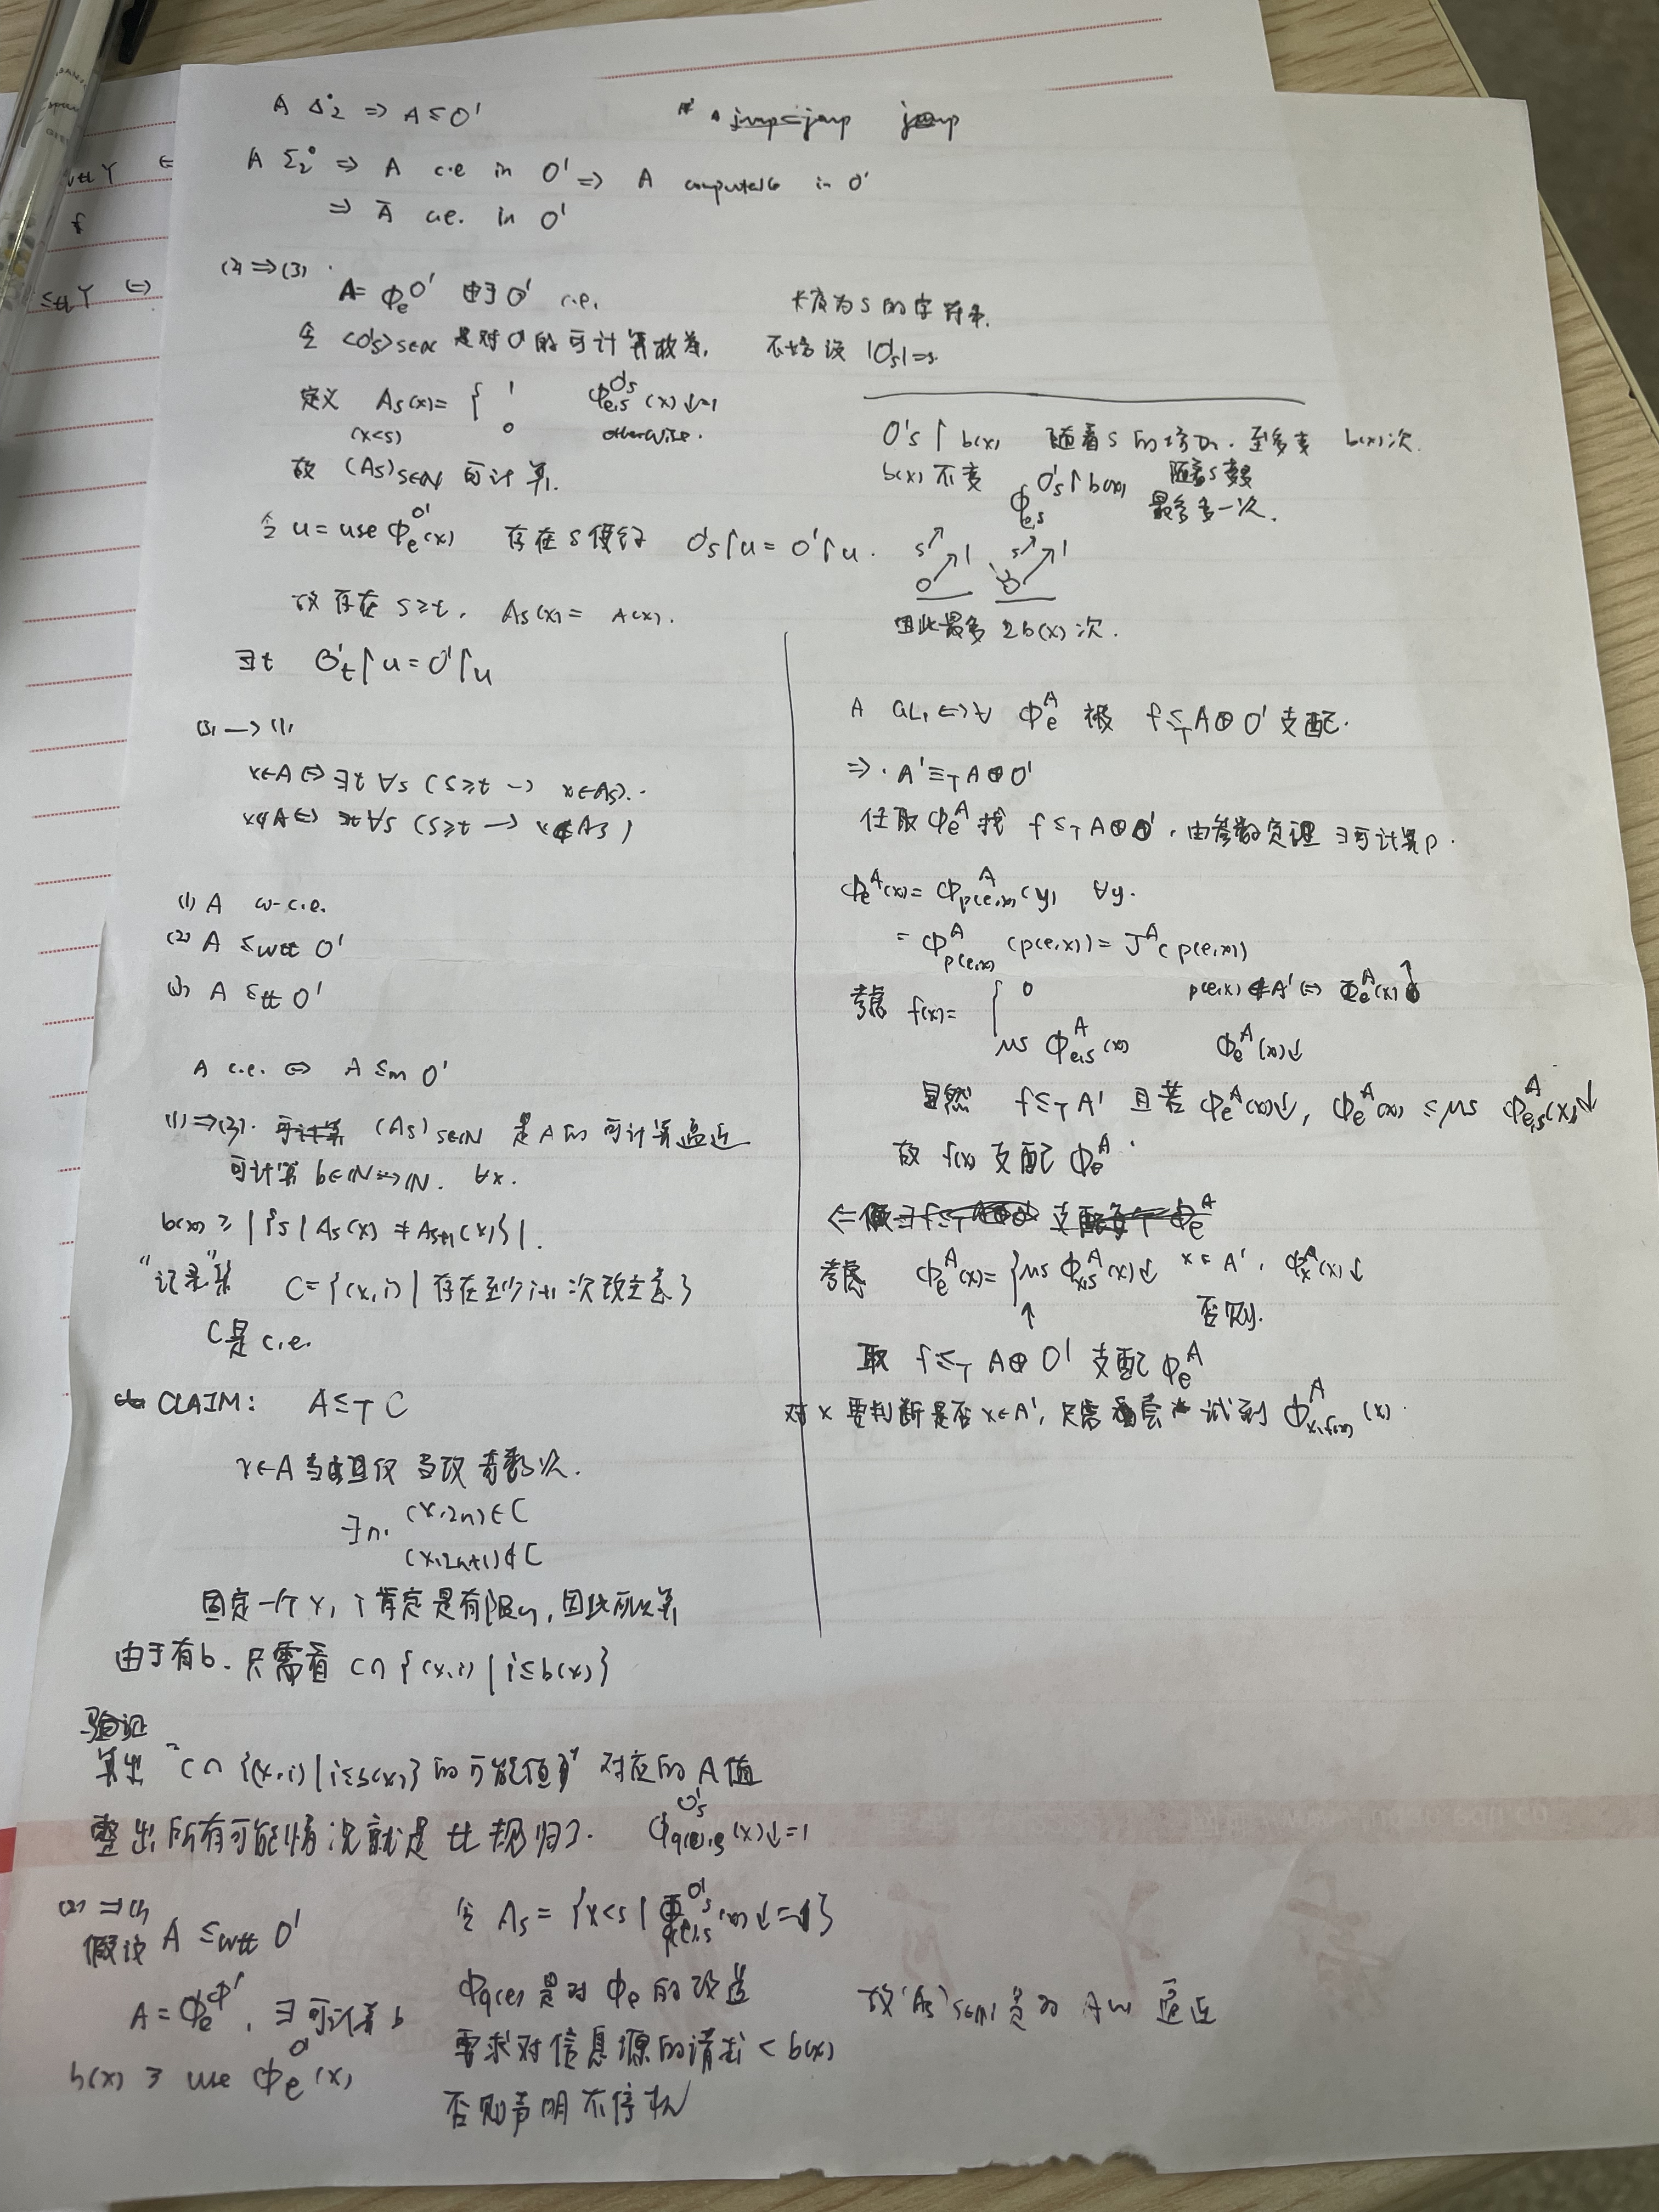
\includegraphics[width=.4\textwidth]{../images/15445/1.png}
\label{}
\end{figure}

The DBMS maintains special pages that tracks the location of data pages in the database files

The directory also records the number of free slots per page

must make sure that the directory pages are in sync with the data pages

\begin{figure}[htbp]
\centering
\includegraphics[width=.4\textwidth]{../images/15445/2.png}
\label{}
\end{figure}
\subsection{Page Layout}
\label{sec:orgbe3cb80}
Every page contains a \textbf{header} of metadata about the page's content
\begin{itemize}
\item page size
\item checksum
\item DBMS version
\item transaction visibility
\item compression information
\end{itemize}
Some systems require pages to be self-contained

For any page storage architecture, we need to decide how to organize the data inside of the page

Two approaches
\begin{itemize}
\item tuple-oriented
\item log-structured
\end{itemize}

\textbf{Tuple-oriented}:

Strawman Idea: keep track of the number of tuples in a page and then just append a new tuple to
the end
\begin{itemize}
\item What happens if we delete a tuple
\item what happens if we have a variable-length attribute
\end{itemize}
\begin{figure}[htbp]
\centering
\includegraphics[width=.4\textwidth]{../images/15445/3.png}
\label{}
\end{figure}

The most common layout scheme is called \textbf{slotted pages}, the slot array maps ``slots'' to the
tuples' starting position offsets

The header keeps track of
\begin{itemize}
\item the \# of used slots
\item The offset of the starting location of the last slot used
\end{itemize}

\begin{figure}[htbp]
\centering
\includegraphics[width=.3\textwidth]{../images/15445/4.png}
\label{}
\end{figure}

The DBMS needs a way to keep track of individual tuples, each tuple is assigned a unique \textbf{record
identifier}
\begin{itemize}
\item most common: \texttt{page\_id} + \texttt{offset/slot}
\end{itemize}

An application cannot rely on these IDs to mean anything
\subsection{Tuple layout}
\label{sec:org9c1d93e}
A tuple is essentially a sequence of bytes

It's the job of the DBMS to interpret those bytes into attribute types and values

Each tuple is prefixed with a \textbf{header} that contains meta-data about it
\begin{itemize}
\item visibility info
\item bit map for \texttt{NULL} values
\end{itemize}

We do \textbf{not} need to store meta-data about the schema

Attributes are typically stored in the order that you specify them when you create the table.

DBMS can physically \textbf{denormalize} (pre join) related tuples and store them together in the same
page
\begin{figure}[htbp]
\centering
\includegraphics[width=.3\textwidth]{../images/15445/5.png}
\label{}
\end{figure}

\begin{figure}[htbp]
\centering
\includegraphics[width=.3\textwidth]{../images/15445/6.png}
\label{}
\end{figure}

Instead of storing tuples in pages, the DBMS only stores \textbf{log records}

The system appends log records to the file of how the database was modified
\begin{itemize}
\item inserts store the entire tuple
\item deletes mark the tuple as deleted
\item updates contain the delta of just the attributes that were modified
\end{itemize}

\begin{figure}[htbp]
\centering
\includegraphics[width=.4\textwidth]{../images/15445/7.png}
\label{}
\end{figure}

To read as records, the DBMS scans the log backwards and ``recreates'' the tuple to find what it
needs

Build indexes to allow it to jump to locations in the log
\begin{figure}[htbp]
\centering
\includegraphics[width=.4\textwidth]{../images/15445/8.png}
\label{}
\end{figure}

Periodically compact the log
\begin{figure}[htbp]
\centering
\includegraphics[width=.4\textwidth]{../images/15445/9.png}
\label{}
\end{figure}

Compaction coalesces larger log files into smaller files by removing unnecessary records
\begin{figure}[htbp]
\centering
\includegraphics[width=.8\textwidth]{../images/15445/10.png}
\label{}
\end{figure}
\subsection{Data representation}
\label{sec:org2432df1}
\begin{itemize}
\item \texttt{INTEGER} / \texttt{BIGINT} / \texttt{SMALLINT} / \texttt{TINYINT}
C/C++ Representation
\item \texttt{FLOAT} / \texttt{REAL} vs. \texttt{NUMERIC} / \texttt{DECIMAL}

IEEE-754 Standard / Fixed-point Decimals

numerical/decimal is accurate without rounding errors
\item \texttt{VARCHAR} / \texttt{VARBINARY} / \texttt{TEXT} / \texttt{BLOB}

Header with length, followed by data bytes.
\item \texttt{TIME} / \texttt{DATE} / \texttt{TIMESTAMP}

32/64-bit integer of (micro)seconds since Unix epoch
\end{itemize}


To store values that are larger than a page, the DBMS uses separate \textbf{overflow} storage pages

\begin{figure}[htbp]
\centering
\includegraphics[width=.4\textwidth]{../images/15445/11.png}
\label{}
\end{figure}

Some systems allow you to store a really large value in an external file, treated as a \texttt{BLOB} type

The DBMS \textbf{cannot} manipulate the contents of an external file

\subsection{system catalogs}
\label{sec:orgcc776e0}
A DBMS stores meta-data about databases in its internal catalogs
\begin{itemize}
\item tables, columns, indexes, views
\item users, permissions
\item internal statistics
\end{itemize}

Almost every DBMS stores the database's catalog inside itself

You can query the DBMS's internal \texttt{INFORMATION\_SCHEMA} catalog to get info about the database

\emph{List all the tables in the current database}:
\begin{minted}[]{sql}
/*SQL-92*/
SELECT *
FROM INFORMATION_SCHEMA.TABLES
WHERE table_catalog = '<db_name>';

/*Postgres*/
\d;

/*MySQL*/
SHOW TABLES;

/*SQLite*/
.tables
\end{minted}

\emph{List all the tables in the student table}
\begin{minted}[]{sql}
/*SQL-92*/
SELECT *
FROM INFORMATION_SCHEMA.TABLES
WHERE table_catalog = 'student';

/*Postgres*/
\dstudent;

/*MySQL*/
DESCRIBE student;

/*SQLite*/
.schema student
\end{minted}

Database workloads:
\begin{itemize}
\item On-line transaction processing (OLTP)

fast operations that only read/update a small amount of data each time
\item On-line analytical processing (OLAP)

complex queries that read a lot of data to compute aggregates
\item Hybrid transaction + analytical processing (HTAP)

OLTP+OLAP together on the same database instancew
\end{itemize}
\subsection{storage models}
\label{sec:orgc8dcffc}
The DBMS cna store tuples in different ways that are better for either OLTP or OLAP workloads

We haven been assuming the \(n\)-ary storage model so fart this semester

\textbf{n-ary storage model (NSM)}: the DBMS stores all attributes for a single tuple contiguously in a
 page

Ideal for OLTP workloads where queries tend to operate only on an individual entity and
insert-heavy workloads

\begin{figure}[htbp]
\centering
\includegraphics[width=.5\textwidth]{../images/15445/12.png}
\label{}
\end{figure}

\begin{figure}[htbp]
\centering
\includegraphics[width=.5\textwidth]{../images/15445/13.png}
\label{}
\end{figure}

Advantages
\begin{itemize}
\item fast insertions, updates and deletes
\item Good for querries that need the entire tuple
\end{itemize}
Disadvantages
\begin{itemize}
\item not good for scanning large portions of the table and/or a subset of the attributes
\end{itemize}

\textbf{decomposition storage model (DSM)}: the DBMS stores the values of a single attribute for all
 tupoles contiguously in a page
\begin{itemize}
\item also known as a ``column store''
\end{itemize}
\begin{figure}[htbp]
\centering
\includegraphics[width=.5\textwidth]{../images/15445/14.png}
\label{}
\end{figure}

Tuple identification:
\begin{itemize}
\item fixed-length offsets

each value is the same length for an atrribute
\item embedded tuple Ids

each value is stored with its tuple id in a column
\end{itemize}
\section{Buffer Pools}
\label{sec:orgce8aed7}
How the DBMS manages its memory and move data back-and-forth from disk

\begin{itemize}
\item spatial control
\begin{itemize}
\item where to write pages on disk
\item the goal is to keep pages that are used together often as physically close together as
possible on disk
\end{itemize}
\item temporal control
\begin{itemize}
\item when to read pages into memory, and when to write them to disk
\item the goal is to minimize the number of stalls from having to read data from disk
\end{itemize}
\end{itemize}
\subsection{Buffer Pool Manager}
\label{sec:org1ebc535}
Memory region organized as an array of fixed-size pages. An array entry is called a \textbf{frame}

When  the DBMS requests a page, an exact copy is places into one of these frames

The \textbf{page table} keeps track of pages that are currently in memory

Also maintains additional meta-data per page
\begin{itemize}
\item dirty flag
\item pin/reference counter
\end{itemize}

\textbf{Locks}
\begin{itemize}
\item protects the database's logical contents from other transactions
\item held for transaction duration
\item need to be able to rollback changes
\end{itemize}

\textbf{Latches}
\begin{itemize}
\item protects the critical sections of the DBMS's internal data structure from other threads
\item held for operation duration
\item do not need to be able to rollback changes
\end{itemize}

The \textbf{page directory} is the mapping from page ids to page locations in the database files
\begin{itemize}
\item all changes must be recorded on disk to allow the DBMS to find on restart
\end{itemize}

The \textbf{page table} is the mapping from page ids to a copy of the page in buffer pool frames
\begin{itemize}
\item this is an in-memory data structure that does not need to be stored on disk
\end{itemize}

Buffer pool optimizations
\begin{itemize}
\item multiple buffer pools
\item pre-fetching
\item scan sharing
\item buffer pool bypass
\end{itemize}
\subsubsection{Multiple Buffer Pools}
\label{sec:org2aff88d}
The DBMS does not always have a single buffer pool for the entire system
\begin{itemize}
\item multiple buffer pool instances
\item per-database buffer pool
\item per-page type buffer pool
\end{itemize}

Helps reduce latch contention and improve locality

Approach 1: Object Id
\begin{itemize}
\item Embed an object identifier in record ids and then maintain a mapping from objects to specific
buffer pools
\end{itemize}

Approach 2: Hashing
\begin{itemize}
\item Hash the page id to select which buffer pool to access
\end{itemize}
\subsubsection{Pre-fetching}
\label{sec:org64c94b4}
The DBMS can also prefetch pages based on query plan
\subsubsection{Scan Sharing}
\label{sec:org6d49502}
Queries can reuse data retrieved from storage or operator computations
\begin{itemize}
\item Also called \textbf{synchronized scans}
\end{itemize}

Allow multiple queries to attach to a single cursor that scans a table
\begin{itemize}
\item queries don't have to be the same
\item can also share intermediate results
\end{itemize}
\subsubsection{Buffer Pool Bypass}
\label{sec:org2418b65}
The sequential scan operator won't store fetched pages in the buffer pool to avoid overhead
\subsection{Replacement Policies}
\label{sec:org5012701}
Least-recently  used

Approximation of LRU that does not need a separate timestamp per page
\begin{itemize}
\item each page has a reference bit
\item when a page is accessed, set to 1
\end{itemize}

Organize the pages in a circular buffer with a clock hand
\begin{itemize}
\item upon sweeping, check if a page's bit is set to 1
\item if yes, set to zero. If no, then evict
\end{itemize}

Better policies:
\begin{itemize}
\item LRU-K

Track the history of last K references to each page as timestamps and compute the interval
between subsequent accesses

The DBMS then uses this history to estimate the next time that page is going to be accessed
\item The DBMS chooses which pages to evict on a per txn/query basis.
\end{itemize}


\subsection{Other Memory Pools}
\label{sec:orgabc241e}
\begin{itemize}
\item sorting + join buffers
\item query caches
\item maintenance buffers
\item log buffers
\item dictionary caches
\end{itemize}
\section{Hashtables}
\label{sec:orge0a0788}
We are now going to talk about how to support the DBMS's execution engine to read/write data
from pages

\subsection{Hash functions}
\label{sec:org5a708f9}
\begin{itemize}
\item crc-64 (1975)
\item murmurhash (2008)
\item google cityhash (2011)
\item facebook xxhash (2012)
\item google farmhash (2014)
\end{itemize}

\subsection{static hashing schemes}
\label{sec:org3ec0644}
\subsubsection{linear probe hashing}
\label{sec:org8c34a26}
single giant table of slots

resolve collisions by linearly searching for the next free slot in the table
\begin{itemize}
\item to determine whether an element is present, hash to a location in the index and scan for it
\item must store the key in the index to know when to stop scanning
\item insertions and deletions are generalizations of lookups
\end{itemize}

delete: support A and B are hashed into the same location and then B is the next element of A,
now if we delete A, how do we find the B
\begin{itemize}
\item tombstone
\item movement
\end{itemize}

For non-unique keys,
\begin{enumerate}
\item separated linked list
\item redundant keys
\end{enumerate}

\begin{figure}[htbp]
\centering
\includegraphics[width=.4\textwidth]{../images/15445/15.png}
\label{}
\end{figure}
\subsubsection{robin hood hashing}
\label{sec:org4e453eb}
Variant of linear probe hashing that steals slots from ``rich'' keys and give them to ``poor'' keys.
\begin{itemize}
\item Each key tracks the number of positions they are from where its optimal position in the table.
\item On insert, a key takes the slot of another key if the first key is farther away from its
optimal position than the second key.
\end{itemize}
\subsubsection{cuckoo hashing}
\label{sec:org9b4ca76}
Use multiple hash tables with different hash functions seeds
\begin{itemize}
\item on insert, check every table and pick anyone that has a free slot
\item if no table has a free slot, evict the element from one of them and then re-hash it find a new
location
\end{itemize}
Look-ups and deletions are always O(1) because only one location per hash table is checked
\subsection{dynamic hashing schemes}
\label{sec:org162683d}
\subsubsection{Chained hashing}
\label{sec:org7f09108}
maintain a linked list of \textbf{buckets} for each slot in the hash table

resolve collisions by replacing all elements with the same hash key into the same bucket
\begin{itemize}
\item to determine whether an element is present, hash to its buckets and scan for it
\end{itemize}
\begin{figure}[htbp]
\centering
\includegraphics[width=.6\textwidth]{../images/15445/16.png}
\label{}
\end{figure}
\subsubsection{extendible hashing}
\label{sec:orgf05763a}
\href{https://emunix.emich.edu/\~shaynes/Papers/ExtendibleHashing/extendibleHashing.html}{better source}

chained-hashing approach where we split buckets instead of letting the linked list grow forever

multiple slot locations can point to the same bucket chain

reshuffle bucket entires on split and increase the number of bits to examine

\begin{figure}[htbp]
\centering
\includegraphics[width=.6\textwidth]{../images/15445/17.png}
\label{}
\end{figure}
\subsubsection{linear hashing}
\label{sec:org5f11f01}
The hash table maintains a \textbf{pointer} that tracks the next bucket to split
\begin{itemize}
\item when any bucket overflows, split the bucket at the pointer location
\end{itemize}

use multiple hashes to find the right bucket for a given key

can use different overflow criterion
\section{Tree Indexes}
\label{sec:orga3f8ea0}
A \textbf{table index} is a replica of a subset of a table's attributes that are organized and/or sorted
for efficient using those attributes
\subsection{B+ Tree overview}
\label{sec:org8127d1b}
B-tree, B+tree, B*tree, Blink-tree

A B+Tree is a self-balancing tree data structure that keeps data sorted and allows searches,
sequential access, insertions and deletions in \(O(\log n)\)
\begin{itemize}
\item optimized for systems that read and write large blocks of data
\end{itemize}

A B+Tree is an \(M\)-way search tree with the following properties
\begin{itemize}
\item it is perfectly balanced (i.e., every leaf node is at the same depth in the tree)
\item every node other than the root is at least half-full \(M/2-1\le\text{\#keys}\le M-1\)
\item every inner node with \(k\)  keys has \(k+1\) non-null children
\end{itemize}
\begin{figure}[htbp]
\centering
\includegraphics[width=.7\textwidth]{../images/15445/18.png}
\label{}
\end{figure}

Every B+Tree node is comprised of an array of key/value pairs
\begin{itemize}
\item the keys are derived from  the attributes that the index is based on
\item the values will differ based on whether the node is classified as an \textbf{inner node} or a \textbf{leaf node}
\end{itemize}

The arrays are (usually) kept in sorted key order

Leaf node values approach
\begin{enumerate}
\item record IDs

A pointer to the location of the tuple to which the index corresponds

\item tuple data

the leaf nodes store the actual contents of the tuple

secondary indexes must store the record ID as their values
\end{enumerate}

\textbf{Insert}
\begin{enumerate}
\item find correct leaf node L
\item put data entry into L in sorted order
\item if L has enough space, done
\item otherwise, split L keys into L and a new node L2
\begin{itemize}
\item redistribute entries evenly, copy up middle key
\item insert index entry pointing to L2 into parent of L
\end{itemize}
\end{enumerate}

\textbf{Delete}
\begin{enumerate}
\item find leaf L where entry belongs. remove the entry
\item if L is at least half-full, done
\item if L has only M/2-1 entries
\begin{itemize}
\item try to re-distribute, borrowing from sibling
\item if re-distribution fails, merge L and sibling
\end{itemize}
\end{enumerate}
If merge occured, must delete entry from parent of L

\textbf{Duplicate keys}
\begin{enumerate}
\item append record ID
\begin{itemize}
\item add the tuple's unique record ID as part of the key to ensure that all keys are unique
\item the DBMS can still use partial keys to find the tuples
\end{itemize}
\item Overflow leaf nodes
\begin{itemize}
\item allow leaf nodes to spill into overflow nodes that contain the duplicate keys
\end{itemize}
\end{enumerate}

\textbf{clustered indexes}
The table is stored in the sort order specified by the primary key
\begin{itemize}
\item can be either heap- or index-organized storage
\end{itemize}

some DBMS always use a clustered index
\begin{itemize}
\item if a table does not contain a primary key, the DBMS will automaticall y make a hidden primary key
\end{itemize}
\subsection{use in a DBMS}
\label{sec:orge792400}
\subsection{Design choices}
\label{sec:orgf515652}
\subsubsection{node size}
\label{sec:org5d337f8}
the slower the storage device, the larger the optimal node size for a B+ Tree
\begin{itemize}
\item HDD: 1MB
\item SSD: 10KB
\item In-Memory: 512B
\end{itemize}

optimal sizes can vary depending on the workload


\subsubsection{merge threshold}
\label{sec:orgdd45f85}
some DBMSs do not always merge nodes when they are half full

delaying a merge operation may reduce the amount of reorganization

it may also be better to just let smaller nodes exist and then periodically rebuild entire tree

\subsubsection{variable-length keys}
\label{sec:org256110a}
\begin{enumerate}
\item pointers
\item variable-length nodes
\item padding
\item key map / indirection
\end{enumerate}
\subsubsection{intra-node search}
\label{sec:orgc81208d}
\begin{enumerate}
\item linear
\item binary
\item interpolation
\end{enumerate}
\subsection{optimizations}
\label{sec:orgb439c9a}
\subsubsection{prefix compression}
\label{sec:org16164dd}
sorted keys in the smae leaf node are likely to have the same prefix
\begin{center}
\begin{tabular}{lll}
robbed & robbing & robot\\
\end{tabular}
\end{center}

Instead of storing the entire key each time, extract common prefix and store only unique suffix
for each key
\subsubsection{deduplication}
\label{sec:orgbcacca5}
non-unique indexes can end up storing multiple copies of the same key in leaf nodes

the leaf node can store the key once and then maintain a list of tuples with that key
\subsubsection{bulk insert}
\label{sec:orge4d7e19}
The fastest way to build a new B+Tree for an existing table is to first sort the keys and then
rebuild the index from the bottom up
\section{Index Concurrency}
\label{sec:orged82767}
\subsection{Latches Overview}
\label{sec:org7e272d7}
\textbf{Locks}
\begin{itemize}
\item protect the database's logical contents from other txns
\item held for txn duration
\item need to be able to rollback changes
\end{itemize}

\textbf{Latches}
\begin{itemize}
\item Protect the critical sections of the DBMS's internal data structure from other threads
\item held for operation duration
\item do not need to be able to rollback changes
\end{itemize}

\begin{center}
\begin{tabular}{lll}
 & Locks & Latches\\
Separate & User Txns & Threads\\
Protect & Database Contents & In-Memory Data Structures\\
During & Entire Txns & Critical Sections\\
Modes & Shared, Exclusive, Update, Intention & Read, Write\\
Deadlock & Detection \& Resolution & Avoidance\\
by & Waits-for, Timeout, Aborts & Coding Discipline\\
Kept in & Lock Manager & Protected Data Structure\\
\end{tabular}
\end{center}

\subsubsection{Latch Modes}
\label{sec:org3a89170}
\textbf{Read Mode}
\begin{itemize}
\item Multiple threads can read the same object at the same time
\item A thread can acquire the read latch if another thread has it in read mode
\end{itemize}

\textbf{Write Mode}
\begin{itemize}
\item Only one thread an access the object
\item A thread cannot acquire a write latch if another thread has it in any mode
\end{itemize}

\subsubsection{Latch Implementations}
\label{sec:orgc771c15}
\begin{enumerate}
\item Blocking OS Mutex
\label{sec:org6608800}
non-scalable (about 25ns per lock/unlock invocation)

\begin{minted}[]{c++}
std::mutex m;

m.lock();

m.unlock();
\end{minted}

But \texttt{std::mutex} -> \texttt{pthread\_mutex\_t} -> \texttt{futex}
\item Test-and-Set Spin Latch (TAS)
\label{sec:org19b383a}
\begin{itemize}
\item very efficient (single instruction to latch/unlatch)
\item non-scalable, not cache-friendly, not OS-friendly
\item \texttt{std::atomic<T>}
\end{itemize}

\begin{minted}[]{c++}
std::atomic_flag latch;

while (latch.test_and_set(...)) {

}
\end{minted}

\textbf{Do not use spinlocks in user space, unless you actually know what you're doing}. And be aware
that the likelihood that you know what you are doing is basically nil.
\item Read-Writer Latches
\label{sec:org11b9c09}
\begin{itemize}
\item Allows for concurrent readers
\item Must manage read/write queues to avoid starvation
\item can be implemented on top of spin latches
\end{itemize}
\end{enumerate}

\subsection{Hash table latching}
\label{sec:org647ed0a}
easy to support concurrent access due to the limited ways threads access the data structure
\begin{itemize}
\item all threads move in the same direction and only access a single page/slot at a time
\item deadlocks are not possible
\end{itemize}

To resize the table, take a global write latch on the entire table

\begin{enumerate}
\item Page latches
\begin{itemize}
\item each page has its own reader-writer latch that protects its entire contents
\item threads acquire either a read or write latch before they access a page
\end{itemize}
\item Slot latches
\begin{itemize}
\item each slot has its own latch
\item can use a single-mode latch to reduce meta-data and computational overhead
\end{itemize}
\end{enumerate}

Atomic instruction that compares contents of a memory location M to a given value V
\texttt{\_\_sync\_bool\_compare\_and\_swap(\&M,20,30)}
\begin{itemize}
\item if values are equal, installs new given value V' in M
\item otherwise operation fails
\end{itemize}

\subsection{B+Tree Latching}
\label{sec:org214068b}
We want to allow multiple threads to read and update a B+ Tree at the same time

We need to protect against two types of problems
\begin{itemize}
\item threads trying to modify the contents of a node at the same time
\item one thread traversing the tree while another thread splits/merge nodes
\end{itemize}
\subsubsection{Latch crabbing/coupling}
\label{sec:org87487f6}
Protocol to allow multiple threads to access/modify B+ Tree at the same time

\textbf{Basic idea}:
\begin{itemize}
\item get latch for parent
\item get latch for child
\item release latch for parent if ``safe''
\end{itemize}

A \textbf{safe node} is one that will not split or merge when updated
\begin{itemize}
\item not full
\item more than half-full
\end{itemize}

\textbf{Find}: start at root and go down
\begin{itemize}
\item acquire R latch on child
\item then unlatch parent
\end{itemize}

\textbf{Insert/Delete}: Start at root and go down, obtaining W latches as needed. Once child is latched,
 check if it is safe:
\begin{itemize}
\item if child is safe, release all latches on ancestors
\end{itemize}

But taking a write latch on the root every time becomes a bottleneck with higher concurrency
\subsubsection{Better latching algorithm}
\label{sec:org8b68ce2}
Most modifications to a B+Tree will \uline{not} require a split or merge

Instead of assuming that there will be a split/merge, optimistically traverse the tree using
read latches

If you guess wrong, repeat traversal with the pessimistic algorithm

\textbf{Search}: same as before

\textbf{Insert/Delete}:
\begin{itemize}
\item set latches as if for search, get to leaf, and set W latch on leaf
\item if leaf is not safe, release all latches, and restart thread using previous insert/delete
protocol with write latches
\end{itemize}

This approach optimistically assumes that only leaf node will be modified; if not, R latches set
on the first pass to leaf are wasteful
\subsection{Leaf Node Scans}
\label{sec:orge329d84}
The threads in all the examples so far have acquired latches in a ``top-down'' manner

But what if we want to move from one leaf node to another leaf node?

Latches do not support deadlock detection or avoidance. The only way we can deal with this
problem is through coding discipline

The leaf node sibling latch acquisition protocol must support a ``no-wait'' mode

The DBMS's data structures must cope with failed latch acquisitions
\section{Sorting \& Aggregations}
\label{sec:org53b09d5}
\subsection{External Mergre Sort}
\label{sec:org4e9c219}
What do we need to sort
\begin{itemize}
\item relational model/SQL is unsorted
\item queries may request that tuples are sorted in a specific way
\item But even if a query does not specify an order, we may still want to sort to do other things
\begin{itemize}
\item trivial to support duplicate elimination
\item bulk loading sorted tuples into a B+ tree index is faster
\item aggregations
\end{itemize}
\end{itemize}
\subsubsection{2-way external merge sort}
\label{sec:orge679916}
2 is the number of runs that we are going to merge into a new run for each pass

data is broken up into N pages

the DBMS has a finite number of B buffer pool pages to hold input and output data

\textbf{Pass 0}
\begin{itemize}
\item read all B pages of the table into memory
\item sort pages into runs and write them back to disk
\end{itemize}

\textbf{Pass 1,2,3,..}
\begin{itemize}
\item recursively merge pairs of runs into runs twice as long
\item uses three buffer pages (2 for input pages, 1 for output)
\end{itemize}

Number of pass: \(1+\lceil\log_2N\rceil\)

Total I/O cost: \(2N\cdot(\#\text{ of passes})\)

\begin{figure}[htbp]
\centering
\includegraphics[width=.6\textwidth]{../images/15445/19.png}
\label{}
\end{figure}

This algorithm only requires three buffer pool pages to perform the sorting

\textbf{Double buffering optimization}
Prefetch the next run in the background and store it in a second buffer while system is
processing the current run
\begin{itemize}
\item reduces the wait time for I/O requests at each step
\end{itemize}
\subsubsection{General external merge sort}
\label{sec:orgaea1789}
\textbf{Pass 0}
\begin{itemize}
\item use B buffer pages
\item produce \(\lceil N/B\rceil\) sorted runs of size B
\end{itemize}

\textbf{Pass 1}
\begin{itemize}
\item merge \(B-1\) runs
\end{itemize}

Number of pass: \(1+\lceil\log_{B-1}\lceil N/B\rceil\rceil\)

Total I/O cost: \(2N\cdot(\#\text{ of passes})\)
\subsubsection{Using B+Trees for sorting}
\label{sec:org3e61a81}

\subsection{Aggregations}
\label{sec:orga6f5f0b}
Two implementation choices
\begin{itemize}
\item sorting
\item hashing
\end{itemize}

\begin{figure}[htbp]
\centering
\includegraphics[width=.8\textwidth]{../images/15445/20.png}
\label{}
\end{figure}

\textbf{Hashing aggregate}: Populate an ephemeral hash table as the DBMS scans the table. For each
 record, check whether there is already an entry in the hash table:
\begin{itemize}
\item \texttt{DISTINCT}: discard duplicate
\item \texttt{GROUP BY}: perform aggregate computation
\end{itemize}

If everything fits in memory, then this is easy


\subsubsection{External hashing aggregate}
\label{sec:org96035a1}
\begin{enumerate}
\item Phase 1: Partition
\label{sec:org77010d8}
\begin{itemize}
\item divide tuples into buckets based on hash key
\item write them out to disk when they get full
\end{itemize}

use a hash function \(h_1\) to split tuples into \textbf{partitions} on disk
\begin{itemize}
\item a partition is one or more pages that contain the set of keys with the same hash value
\item partitions are ``spilled'' to disk via output buffers
\end{itemize}

Assume that we have B buffers, we will use B-1 buffers for the partitions and 1 buffer for the
input data

\begin{figure}[htbp]
\centering
\includegraphics[width=.8\textwidth]{../images/15445/21.png}
\label{}
\end{figure}

\item Phase 2: ReHash
\label{sec:orge35451d}
\begin{itemize}
\item build in-memory hash table for each partition and compute the aggregation
\end{itemize}

For each partition on disk
\begin{itemize}
\item read it into memory and build an in-memory hash table based on a second hash function \(h_2\)
\item then go through each bucket of this hash table to bring together matching tuples
\end{itemize}

This assumes that each partition fits in memory
\end{enumerate}

\subsubsection{Hashing summarization}
\label{sec:org0ec0cce}
During the rehash phase, store pairs of the form \texttt{GroupKey->RunningVal}

when we want to insert a new tuple into the hash table
\begin{itemize}
\item if we find a matching \texttt{GroupKey}, just update the \texttt{RunningVal} appropriately
\item else insert a new \texttt{GroupKey->RunningVal}
\end{itemize}

\begin{figure}[htbp]
\centering
\includegraphics[width=.8\textwidth]{../images/15445/22.png}
\label{}
\end{figure}


\section{Joins}
\label{sec:org38a6308}
We will focus on performing binary joins (two tables) using \textbf{inner equijoin} algorithms
\begin{itemize}
\item these algorithms can be tweaked to support other joins
\item multi-way joins exist primarily in research literature
\end{itemize}

In general, we want the smaller table to always be the left table (``outer table'') in the query
plan

\textbf{Decision 1}: output
\begin{itemize}
\item what data does the join operator emit to its parent operator in the query plan tree
\end{itemize}

\textbf{Decision 2}: cost analysis criteria
\begin{itemize}
\item how do we determine whether one join algorithm is better than another
\end{itemize}

\begin{minted}[]{sql}
SELECT R.id, S.cdate
  FROM R JOIN S
    ON R.id = S.id
 WHERE S.value > 100
\end{minted}

\begin{figure}[htbp]
\centering
\includegraphics[width=.3\textwidth]{../images/15445/23.png}
\label{}
\end{figure}

For tuple \(r\in R\) and tuple \(s\in S\) that match on join attributes, concatenate \(r\) and \(s\)
together into a new tuple

output contents can vary:
\begin{itemize}
\item depends on processing model
\item depends on storage model
\item depends on data requirements in query
\end{itemize}

\textbf{Early Materialization}:
\begin{itemize}
\item copy the values for the attributes in outer and inner tuples into a new output tuple
\item subsequent operators in the query plan never need to go back to the base tables to get more
data
\end{itemize}

\textbf{Late Materialization}:
\begin{itemize}
\item only copy the joins keys along with the Record IDs of the matching tuples
\item ideal for column stores because the DBMS does not copy data that is not needed for the query
\end{itemize}

\textbf{Cost Analysis Criteria}

Assume
\begin{itemize}
\item \(M\) pages in table \(R\), \(m\) tuples in \(R\)
\item \(N\) pages in table \(S\), \(n\) tuples in \(S\)
\end{itemize}

\textbf{Cost Metric}: \# of IOs to compute join

\(R\bowtie S\) is the most common operation and thus must be carefully optimized

\(R\times S\) followed by a selection is inefficient because the cross-product is large

\subsection{Join algorithms}
\label{sec:orgb6def70}

\subsubsection{Nested Loop Join}
\label{sec:org0cad225}
\begin{enumerate}
\item Simple/Stupid
\label{sec:org8acabf7}
foreach tuple \(r\in R\):
    foreach tuple \(s\in S\):
        emit, if \(r\) and \(s\) match

Cost: \(M+m\cdot N\)
\item Block
\label{sec:org305127f}
foreach block \(B_R\in R\)
    foreach block \(B_S\in S\)
        foreach tuple \(r\in B_r\)
            foreach tuple \(s\in B_s\)
                emit, if \(r\) and \(s\) match

cost: \(M+M\cdot N\)

What if we have B buffers available?
\begin{itemize}
\item use \(B-2\) buffers for scanning the outer table
\item use one buffer for the inner table, one buffer for storing output
\end{itemize}

foreach \(B-2\) blocks \(b_R\in R\)
    foreach block \(b_S\in S\)
        foreach tuple \(r\in B-2\) blocks
            foreach tuple \(s\in b_S\)
                emit, if \(r\) and \(s\) match

Cost: \(M+\lceil M/(B-2)\rceil\cdot N\)
\item Index
\label{sec:orga0f240c}
Why is the basic nested loop join so bad?
\begin{itemize}
\item for each tuple in the outer table, we must do a sequential scan to check for a match in the
inner table
\end{itemize}

We can avoid sequential scans by using an index to find inner table matches
\begin{itemize}
\item use an existing index for the join
\end{itemize}

foreach tuple \(r\in R\)
    for each tuple \(s\in\text{Index}(r_i=s_j)\)
        emit, if \(r\) and \(s\) match
\end{enumerate}
\subsubsection{Sort-Merge Join}
\label{sec:org59efbe5}
\textbf{Phase 1}: sort
\begin{itemize}
\item sort both tables on the join keys
\end{itemize}

\textbf{Phase 2}: merge
\begin{itemize}
\item step through the two sorted tables with cursors and emit matching tuples
\item may need to backtrack depending on the join type
\end{itemize}

sort \(R,S\) on join keys
\(\text{cursor}_S\leftarrow R_{\text{sorted}}\), \(\text{cursor}_S\leftarrow S_{\text{sorted}}\)
while \(\text{cursor}_R\) and \(\text{cursor}_S\):
    if \(\text{cursor}_R>\text{cursor}_S\)
        increment \(\text{cursor}_S\)
    if \(\text{cursor}_R<\text{cursor}_S\)
        increment \(\text{cursor}_R\)
    elif \(\text{cursor}_R\) and \(\text{cursor}_S\) match:
        emit
        increment \(\text{cursor}_S\)


Sort Cost(R): \(2M\cdot(1+\lceil\log_{B-1}\lceil M/B\rceil\rceil)\)
Sort Cost(S): \(2N\cdot(1+\lceil\log_{B-1}\lceil N/B\rceil\rceil)\)
Merge Cost: \(M+N\)

When is sort-merge join useful?
\begin{itemize}
\item one or both tables are already sorted on join key
\item output must be sorted on join key
\item the input relations may be sorted either by an explicit sort operator, or by scanning the
relation using an index on the join key
\end{itemize}
\subsubsection{Hash Join}
\label{sec:org6dcd3a0}
if tuple \(r\in R\) and a tuple \(s\in S\) satisfy the join condition, then they have the same value
for the join attributes

if that value is hashed to some partition \(i\), the \(R\) tuple must be in \(r_i\) and the \(S\)
tuple in \(s_i\)

Therefore \(R\) tuples in \(r_i\) need only to be compared with \(S\) tuples in \(s_i\)

\textbf{Phase 1}: build
\begin{itemize}
\item scan the outer relation and populate a hash table using the hash function \(h_1\) on the join
attributes
\end{itemize}

\textbf{Phase 2}: probe
\begin{itemize}
\item scan the inner relation and use \(h_1\) on each tuple to jump to a location in the hash table
and find a matching tuple
\end{itemize}

Hash table contents

key: the attributes

value: varies per implementation
\begin{itemize}
\item depends on what the operators above the join in the query plan expect as its input
\end{itemize}

\textbf{Approach 1}: full tuple

\textbf{Approach 2}: tuple identifier
\begin{itemize}
\item could be to either the base tables or the intermediate output from child operators in the
query plan
\item ideal for column stores because the DBMS does not fetch data from disk that it does not need
\item also better if join selectivity is low
\end{itemize}

\textbf{Probe phase optimization}:
create a \textbf{Bloom Filter} during the build phase when the key is likely to not exist in the hash
table
\begin{itemize}
\item threads check the filter before probing the hash table. This will be faster since the filter
will fit in CPU caches
\item sometimes called \textbf{sideways information passing}
\end{itemize}


\textbf{Bloom filters} is a probalistic data structure (bitmap) that answers set membership queries
\begin{itemize}
\item false negatives will never occur
\item false positives can sometimes occur
\end{itemize}


\texttt{Insert(x)}: use \(k\) hash functions to set bits in the filter to 1

\texttt{Lookup(x)}: check whether the bits are 1 for each hash function

how big of a table can we hash using this approach?
\begin{itemize}
\item \(B-1\) ``spill partitions'' in phase 1
\item each should be no more than B blocks big
\end{itemize}


Answer: \(B\cdot(B-1)\)
\begin{itemize}
\item a table of \(N\) pages needs about \(\sqrt{N}\) buffers
\item assume hash distributes records evenly. Use a ``fudge factor'' \(f>1\) for that: we
need \(B\cdot\sqrt{fN}\)
\end{itemize}

What happens if we do not have enough memory to fit the entire hash table?

we do not want to let the buffer pool manager swap out the hash table pages at random

Hash join when tables do not fit in memory
\begin{itemize}
\item Build Phase: Hash both tables on the join attribute into partitions
\item Probe Phase: Compares tuples in corresponding partitions for each table
\end{itemize}

Cost: \(3(M+N)\)

partition: \(2(M+N)\)

probing \(M+N\)

\begin{center}
\begin{tabular}{ll}
algorithm & IO cost\\
simple nested loop join & \(M+(m\cdot N)\)\\
block nested loop join & \(M+(M\cdot N)\)\\
index nested loop join & \(M+(M\cdot C)\)\\
Sort-Merge join & \(M+N+\)sort cost\\
hash join & \(3(M+N)\)\\
\end{tabular}
\end{center}
\section{Query execution 1}
\label{sec:org53dcc32}
\subsection{Processing Models}
\label{sec:org549759b}
A DBMS's \textbf{processing model} defines how the system executes a query plan
\begin{itemize}
\item different trade-offs for different workloads
\end{itemize}
\subsubsection{Iterator Model}
\label{sec:org8746617}
Each query plan operator implements a \texttt{next()} function
\begin{itemize}
\item on each invocation, the operator returns either a single tuple or a \texttt{null} marker if there are
no more tuples
\item the operator implements a loop that call \texttt{next()} on its children to retrieve their tuples and
then process them
\end{itemize}
Also called \textbf{volcano} or \textbf{pipeline} model

\begin{figure}[htbp]
\centering
\includegraphics[width=.8\textwidth]{../images/15445/24.png}
\label{}
\end{figure}

This is used in almost every DBMS. Allows for tuple \textbf{pipelining}

some operators must block until their children emit all their tuples
\begin{itemize}
\item joins, subqueries, order by
\end{itemize}

output control works easily with this approach
\subsubsection{Materialization Model}
\label{sec:orgf0b20c0}
Each operator processes its input all at once and then emits its output all at once
\begin{itemize}
\item the operator ``materializes'' its output as a single result
\item the BDMS can push down hints (e.g. \texttt{LIMIT}) to avoid scanning too many tuples
\item can send either a materialized row or a single column
\end{itemize}

The output can be either whole tuples (NSM) or subsets of columns (DSM)
\begin{figure}[htbp]
\centering
\includegraphics[width=.8\textwidth]{../images/15445/25.png}
\label{}
\end{figure}

better for OLTP workloads because queries only access a small number of tuples at a time
\begin{itemize}
\item lower execution / coordinaten overhead
\item fewer function calls
\end{itemize}

not good for OLAP queires with large intermediate results
\subsubsection{Vectorized/Batch Model}
\label{sec:org53f7757}
like the iterator model where each operator implements a \texttt{next()} function, but

each operator emits a \textbf{batch} of tuples instead of single tuple
\begin{itemize}
\item the operator's internal loop processes multiple tuples at a time
\item the size of the batch can vary based on hardware or query properties
\end{itemize}
\begin{figure}[htbp]
\centering
\includegraphics[width=.8\textwidth]{../images/15445/26.png}
\label{}
\end{figure}
Ideal for OLAP queries because it greatly reduces the number of invocations per operator

Allows for operators to more easily use vectorized (SIMD) instructions to process batches of
tuples

\textbf{Plan processing direction}
\begin{itemize}
\item top-to-bottom
\begin{itemize}
\item start with the root and ``pull'' data up from its children
\item tuples are always passed with function calls
\end{itemize}
\item bottom-to-top
\begin{itemize}
\item start with leaf nodes and push data to their parents
\item allows for tighter control of caches/registers in pipelines
\end{itemize}
\end{itemize}
\subsection{Access Methods}
\label{sec:orgc872b9f}
An \textbf{access method} is the way that the DBMS accesses the data stored in a table
\begin{itemize}
\item not defined in relational algebra
\end{itemize}
\subsubsection{Sequential scan}
\label{sec:orgbeb0744}
for each page in the table
\begin{itemize}
\item retrieve it from the buffer pool
\item iterate over each tuple and check whether to include it
\end{itemize}

for page in table.pages:
    for t in page.tuples:
        if evalPred(t)
            // do something

The DBMS maintains an internal \textbf{cursor} that tracks the last page/slot it examined

\textbf{optimizations}:
\begin{itemize}
\item prefetching
\item buffer pool bypass
\item parallelization
\item heap clustering
\item zone maps
\item late meterialization
\end{itemize}

\textbf{zone maps}:
pre-computed aggregates for the attributes values in a page. DBMS checks the zone map first to
decide whether it wants to access the page

\begin{figure}[htbp]
\centering
\includegraphics[width=.5\textwidth]{../images/15445/27.png}
\label{}
\end{figure}

\textbf{late meterialization}:
DSM DBMSs can delay stitching together tuples until the upper parts of the query plan

\begin{figure}[htbp]
\centering
\includegraphics[width=.6\textwidth]{../images/15445/28.png}
\label{}
\end{figure}
\subsubsection{Index scan}
\label{sec:org607bffd}
The DBMS picks an index to find the tuples that the query needs

which index to use depends on
\begin{itemize}
\item what attributes the index contains
\item what attributes the query references
\item the attribute's value domains
\item predicate composition
\item whether the index has unique or non-unique keys
\end{itemize}

suppose that we have a single table with 100 tuples and two indexes: \texttt{age}, \texttt{dept}
\begin{minted}[]{sql}
SELECT * FROM students
 WHERE age < 30
   AND dept = 'CS'
   AND country = 'US'
\end{minted}

scenario 1: there are 99 people under the age of 30 but only 2 people in the CS department

scenario 2: there are 99 people in the CS department but only 2 people under the age of 30

if there are multiple indexes that the DBMS can use for a query:
\begin{itemize}
\item compute sets of Record IDs using each matching index
\item Combine these sets based on the query's predicates (union vs. intersect)
\item retrieve the records and apply any remaining predicates
\end{itemize}

Postgres calls this \textbf{Bitmap Scan}

With an index on \texttt{age} and an index on \texttt{dept}
\begin{itemize}
\item we can retrieve the Record IDs satisfying \texttt{age<30} using the first
\item then retrieve the Record IDs satisfying \texttt{dept='CS'} using the second
\item take their intersection
\item retrieve records and check \texttt{country='US'}
\end{itemize}

set intersection can be done with bitmaps, hash tables, or Bloom filters
\subsection{Modification Queries}
\label{sec:org6c5d470}
Operators that modify the database (\texttt{INSERT}, \texttt{UPDATE}, \texttt{DELETE}) are responsible for checking the
constraints and updating indexes

\texttt{UPDATE/DELETE}:
\begin{itemize}
\item child operators pass Record IDs for the target tuples
\item must keep track of previously seen tuples
\end{itemize}

\texttt{INSERT}:
\begin{itemize}
\item choice 1: materialize tuples inside of the operator
\item choice 2: operator inserts any tuple passed in from child operators
\end{itemize}

Halloween Problem: anomaly where an update operation changes the physical location of a tuple,
which causes a scan operator to visit the tuple multiple times
\subsection{Expression Evaluation}
\label{sec:org8052bb4}
The DBMS represents a \texttt{WHERE} clause as an \textbf{expression tree}

\begin{minted}[]{sql}
SELECT R.id, S.cdata
  FROM R JOIN S
    ON R.id = S.id
 WHERE S.value > 100
\end{minted}

The nodes in the tree represent different expression types:
\begin{itemize}
\item comparisons (\texttt{=}, \texttt{<}, \texttt{>}, \texttt{!=})
\item conjunctions \texttt{AND}, disjunction \texttt{OR}
\item arithmetic operators (\texttt{+}, \texttt{-}, \texttt{*}, \texttt{/}, \texttt{\%})
\item constant values
\item tuple attribute references
\end{itemize}

\begin{figure}[htbp]
\centering
\includegraphics[width=.7\textwidth]{../images/15445/29.png}
\label{}
\end{figure}

\begin{figure}[htbp]
\centering
\includegraphics[width=.8\textwidth]{../images/15445/30.png}
\label{}
\end{figure}
\section{Query Execution 2}
\label{sec:orgd5cf722}
Parallel DBMSs
\begin{itemize}
\item resources are physically close to each other
\item resources communicate over high-speed interconnect
\item communication is assumed to be cheap and reliable
\end{itemize}

Distributed DBMSs
\begin{itemize}
\item resources can be far from each other
\item resources communicate using slow interconnect
\item communication cost and problems cannot be ignored
\end{itemize}
\subsection{Process Models}
\label{sec:org498cb51}
A DBMS's \textbf{process model} defines how the system is architected to support concurrent requests from
a multi-user application

A \textbf{worker} is the DBMS component that is responsible for executing tasks on behalf of the client
and returning the results
\begin{enumerate}
\item Process per DBMS Worker

each worker is a separate OS process
\begin{itemize}
\item relies on OS scheduler
\item use shared-memory for global data structures
\item a process crash doesn't take down entire system
\item examples: IBM DB2, Postgres, oracle
\end{itemize}
\item Process Pool

a worker uses any free process from the pool
\begin{itemize}
\item still relies on OS scheduler and shared memory
\item bad for cpu cache locality
\item examples: IBM DB2, Postgres(2015)
\end{itemize}
\item Thread per DBMS Worker

single process with multiple worker threads
\begin{itemize}
\item DBMS manages its own scheduling
\item may or may not use a dispatcher thread
\item thread crash (may) kill the entire system
\item examples: IBM DB2, MSSQL, MySQL, Oracle(2014)
\end{itemize}
\end{enumerate}


Advantages of a multi-threaded architecture
\begin{itemize}
\item less overhead per context switch
\item do not have to manage shared memory
\end{itemize}

The thread per worker model does \textbf{not} mean that the DBMS supports intra-query parallelism

For each query plan, the DBMS decides where, when, and how to execute it
\begin{itemize}
\item how many tasks should i use
\item how many CPU cores should it use
\item what CPU core should the tasks execute on
\item where should a task store its output
\end{itemize}

The DBMS \textbf{always} knows more than the OS

\textbf{Inter-query}: different queries are executed concurrently
\begin{itemize}
\item increases throughput and reduces latency
\item if queries are read-only, then this requires little coordination between queries
\item if multiple queries are updating the database at the same time, then this is hard to do correctly
\end{itemize}

\textbf{Intra-query}: execute the operations of a single query in parallel
\begin{itemize}
\item decreases latency for long-running queries
\item think of organization of operators in terms of \textbf{producer/consumer} paradigm
\item there are parallel versions of every operator: can either have multiple threads access
centralized data structures or use partitioning to divide work up
\end{itemize}

e.g., for parallel grace hash join, use a separate worker to perform the join for each level of
buckets for \(R\) and \(S\) after partitioning

\textbf{intra-query parallelism}:
\subsubsection{intra-operator (horizontal)}
\label{sec:orgb6eed0f}
decompose operators into independent \textbf{fragments} that perform the same function on different
subsets of data

the DBMS inserts an \textbf{exchange} operator into the query plan to coalesce/split results from
multiple children/parent operators

\begin{figure}[htbp]
\centering
\includegraphics[width=.7\textwidth]{../images/15445/31.png}
\label{}
\end{figure}

\textbf{exchange operator}
\begin{enumerate}
\item exchange type 1 - \textbf{gather}: combine the results from multiple workers into a single output stream
\item exchange type 2 - \textbf{distribute}: split a single stream into multiple output streams
\item exchange type 3 - \textbf{repartition}: shuffle multiple input streams across multiple output streams
\end{enumerate}

\begin{figure}[htbp]
\centering
\includegraphics[width=.4\textwidth]{../images/15445/32.png}
\label{}
\end{figure}

\begin{figure}[htbp]
\centering
\includegraphics[width=.7\textwidth]{../images/15445/33.png}
\label{}
\end{figure}
\subsubsection{inter-operator (vertical)}
\label{sec:orge1dff11}
operations are overlapped in order to pipeline data from one stage to the next without
materialization

workers execute operators from different segments of a query plan at the same time

also called \textbf{pipeline parallelism}

\begin{figure}[htbp]
\centering
\includegraphics[width=.6\textwidth]{../images/15445/34.png}
\label{}
\end{figure}
\subsubsection{bushy}
\label{sec:orgdeb4ab2}
bybrid of intra- and inter-operator parallelism where workers execute multiple operators from
different segments of a query plan at the same time

still need exchange operators to combine intermediate results from segments

for
\begin{minted}[]{sql}
SELECT *
FROM A JOIN B JOIN C JOIN D
\end{minted}

\begin{figure}[htbp]
\centering
\includegraphics[width=.4\textwidth]{../images/15445/35.png}
\label{}
\end{figure}
\subsection{Execution Parallelism}
\label{sec:orgcbc3a32}
\subsubsection{I/O parallelism}
\label{sec:org9f5bf48}
split the DBMS across multiple storage devices
\begin{itemize}
\item multiple disks per database
\item one database per disk
\item one relation per disk
\item split relation across multiple disks
\end{itemize}

partitioning: split single logical table into disjoint physical segments that are stored/managed
separately

partitioning should be transparent to the application
\begin{itemize}
\item the application should only access logical tables and not have to worry about how things are
physically stored
\end{itemize}

\textbf{vertical partitioning}: store a table's attributes in a separate location


\subsection{I/O Parallelism}
\label{sec:org005c317}
\section{Optimization 1}
\label{sec:org7e12a23}
\textbf{Heuristics/Rules}
\begin{itemize}
\item rewrite the query to remove stupid/inefficient things
\item these techniques may need to examine catalog, but they do \textbf{not} need to examine data
\end{itemize}

\textbf{Cost-based search}
\begin{itemize}
\item use a model to estimate the cost of executing a plan
\item evaluate multiple equivalence plans for a query and pick the one with the lowest cost
\end{itemize}

\begin{figure}[htbp]
\centering
\includegraphics[width=.7\textwidth]{../images/15445/37.png}
\label{}
\end{figure}

the optimizer generates a mapping of a logical algebra expression to the optimal equivalent
physical algebra expression

physical operators define a specific execution strategy using an access path
\begin{itemize}
\item they can depend on the physical format of the data that they process
\item not always a 1:1 mapping from logical to physical
\end{itemize}

query optimization is NP-Hard
\subsection{Relational Algebra Equivalences}
\label{sec:orgc6d979a}
Two relational algebra expressions are \textbf{equivalent} if they generate the same set of tuples

This is often called \textbf{query rewriting}

\begin{minted}[]{sql}
SELECT s.name, e.cid
  FROM student AS s, enrolled AS e
 WHERE s.sid = e.sid
   AND e.grade = 'A'
\end{minted}
\(\pi_{\text{name},\text{cid}}(\sigma_{\text{grade='A'}}(\text{student}\bowtie\text{enrolled}))\),
which is equivalent to
\(\pi_{\text{name},\text{cid}}(\text{student}\bowtie(\sigma_{\text{grade='A'}}(\text{enrolled})))\),

\textbf{Selections}:
\begin{itemize}
\item perform filters as early as possible
\item break a complex predicate, and push down
\begin{equation*}
\sigma_{p_1\wedge\dots\wedge p_n}(R)=\sigma_{p_1}(\sigma_{p_2}(\dots\sigma_{p_n}(R)))
\end{equation*}
\end{itemize}

\textbf{Joins}:
\begin{itemize}
\item commutative, associative
\end{itemize}

The number of different join orderings for an \(n\)-way join is a \textbf{Catalan Number}

\textbf{Projections}:
\begin{itemize}
\item perform them early to create smaller tuples and reduce intermediate results
\item project out all attributes except the ones requested or required
\end{itemize}

\begin{figure}[htbp]
\centering
\includegraphics[width=.5\textwidth]{../images/15445/38.png}
\label{}
\end{figure}
\subsection{Logical Query Optimization}
\label{sec:org32c2d3e}
Transform a logical plan into an equivalent logical plan using pattern matching rules

The goal is to increase the likelihood of enumerating the optimal plan in the search
\subsubsection{Split Conjunctive Predicates}
\label{sec:orge701206}
Consider
\begin{minted}[]{sql}
SELECT ARTIST.NAME
  FROM ARTIST, APPEARS, ALBUM
 WHERE ARTIST.ID = APPEARS.ARTIST_ID
   AND APPEARS.ALBUM_ID = ALBUM.ID
   AND ALBUM.NAME="Andy's OG Remix"
\end{minted}

Decompose predicates into their simplest forms to make it easier for the optimizer to move them
around
\begin{figure}[htbp]
\centering
\includegraphics[width=.4\textwidth]{../images/15445/39.png}
\label{}
\end{figure}
\subsubsection{Predicate Pushdown}
\label{sec:org7822df4}
Move the predicate to the lowest applicable point in the plan
\begin{figure}[htbp]
\centering
\includegraphics[width=.5\textwidth]{../images/15445/40.png}
\label{}
\end{figure}
\subsubsection{Replace Cartesian Products with Joins}
\label{sec:org9dbd718}
Replace all Cartesian Products with inner joins using the join predicates
\begin{figure}[htbp]
\centering
\includegraphics[width=.5\textwidth]{../images/15445/41.png}
\label{}
\end{figure}
\subsubsection{Projection Pushdown}
\label{sec:orgf86b42c}
Eliminate redundant attributes before pipeline breakers to reduce materialization cost
\begin{figure}[htbp]
\centering
\includegraphics[width=.5\textwidth]{../images/15445/42.png}
\label{}
\end{figure}
\subsection{Nested Queries}
\label{sec:org375cd7c}
The DBMS treats nested sub-queries in the where clause as functions that take parameters and
return a single value or set of values

Two approaches
\begin{itemize}
\item rewrite to de-correlate and/or flattern them
\item decompose nested query and store result to temporary table
\end{itemize}
\subsubsection{Rewrite}
\label{sec:org3c2c0c0}
\begin{minted}[]{sql}
SELECT name FROM sailors AS S
 WHERE EXISTS (
    SELECT * FROM reserves AS R
     WHERE S.sid = R.sid
       AND R.day = '2018-10-15'
)
\end{minted}

\begin{minted}[]{sql}
SELECT name
  FROM sailors AS S, reserves AS R
 WHERE S.sid = R.sid
   AND R.day = '2018-10-15'
\end{minted}
\subsubsection{Decompose}
\label{sec:org08c674f}
\begin{minted}[]{sql}
SELECT S.sid, MIN(R.day)
FROM sailors S, reserves R, boats B
WHERE S.sid = R.sid
AND R.bid = B.bid
AND B.color = 'red'
AND S.rating = (SELECT MAX(S2.rating)
GROUP BY S.sid HAVING COUNT(*) > 1
\end{minted}
For each sailor with the highest rating (over all sailors) and at least two reservations for red
boats, find the sailor id and the earliest data on which the sailor has a reservation for a red
boat

For harder queries, the optimizer breaks up queries into blocks and then concentrate on one
block at a time. Sub-queries are written to a temporary table that are discarded after the query finishes
\subsection{Expression Rewriting}
\label{sec:orgaf9e07c}
An optimizer transforms a query's expressions (e.g., \texttt{WHERE} clause predicates) into the
optimal/minimal set of expressions

Implemented using if/then/else clauses or a pattern-matching rule engine
\begin{itemize}
\item search for expressions that match a pattern
\item when a match is found, rewrite the expression
\item halt if there are no more rules that match
\end{itemize}

Impossible/unnecessary predicates

join elimination
\begin{minted}[]{sql}
SELECT A1.*
  FROM A AS A1 JOIN A AS A2
    ON A1.id = A2.id;
\end{minted}

join elimination with sub-query
\begin{minted}[]{sql}
SELECT * FROM A AS A1
 WHERE EXISTS (SELECT val FROM A AS A2
                WHERE A1.id = A2.id);
\end{minted}

merging predicates
\begin{minted}[]{sql}
SELECT * FROM A
 WHERE val BETWEEN 1 AND 100
    OR val BETWEEN 50 AND 150;
\end{minted}
\subsection{Cost Model}
\label{sec:org2f694d4}
\begin{enumerate}
\item Physical costs
\begin{itemize}
\item predict CPU cycles, I/O, cache misses, RAM consumption, pre-fetching, etc
\item depends heavily on hardware
\end{itemize}
\item logical costs
\begin{itemize}
\item estimate result sizes per operator
\item independent of the operator algorithm
\item need estimations for operator result sizes
\end{itemize}
\item algorithmetic costs
\end{enumerate}

\textbf{disk-based DBMS cost model}: the number of disk accesses will always dominate the execution time
 of a query
\begin{itemize}
\item CPU costs are negligible
\item must consider sequential vs. random I/O
\end{itemize}

The is easier to model if the DBMS has full control over buffer management

postgres cost model: use a combination of CPU and I/O costs that are weighted by ``magic''
constant factors

default settings are for a disk-resident database without a lot of memory
\begin{itemize}
\item processing a tuple in memory is 400x faster than reading a tuple from disk
\item sequential I/O is 4x faster than random I/O
\end{itemize}

IBM DB2 cost model:
\begin{itemize}
\item database characteristics in system catalogs
\item hardware environment
\item storage device characteristics
\item communications bandwidth
\item memory resources
\item concurrency environment
\end{itemize}
\subsection{More cost estimation}
\label{sec:org242b298}
The DBMS stores internal statistics about tables, attributes, and indexes in its internal
catalog

different systems update them at different times

manual invocations:
\begin{itemize}
\item postgres/sqlite: \texttt{ANALYZE}
\item oracle/mysql: \texttt{ANALYZE TABLE}
\item SQL server: \texttt{UPDATE STATISTICS}
\item DB2: \texttt{RUNSTATS}
\end{itemize}

For each relation \(R\), the DBMS maintains the following information
\begin{itemize}
\item \(N_R\): number of tuples in \(R\)
\item \(V(A,R)\): number of distinct values for attribute \(A\)
\end{itemize}

The \textbf{selection cardinality} \(SC(A,R)\) is the average number of records with a value for an
attribute \(A\) given \(N_R/V(A,R)\)

Equality predicates on unique keys are easy to estimate
\begin{minted}[]{sql}
SELECT * FROM people
 WHERE id = 123
\end{minted}
computing the logical cost of complex predicates is more difficult
\begin{minted}[]{sql}
SELECT * FROM people
 WHERE val > 1000
\end{minted}

The \textbf{selectivity} (\texttt{sel}) of a predicate \(P\) is the fraction of tuples that qualify

Formula depends on type of predicate:
\begin{itemize}
\item equality
\item range
\item negation
\item conjunction
\item disjunction
\end{itemize}

Assume that \texttt{V(age,people)} has five distinct values (0-4) and \(N_R=5\)

\textbf{Equality Predicate}: \texttt{A=constant}
\begin{itemize}
\item \(sel(A=constant)=SC(P)/N_R\)
\end{itemize}

\textbf{Range Predicate}:
\begin{itemize}
\item \(sel(A\ge a)=(A_{max}-a+1)/(A_{max}-A_{min}+1)\)
\end{itemize}

\textbf{Negation Query}:
\begin{itemize}
\item \(sel(\neg P)=1-sel(P)\)
\end{itemize}

\textbf{Conjunction}:
\begin{itemize}
\item \(sel(P_1\wedge P_2)=sel(P_1)\cdot sel(P_2)\)
\item assumes predicates are \textbf{independent}
\end{itemize}

\textbf{Disjunction}:
\begin{itemize}
\item \(sel(P_1\vee P_2)=sel(P_1)+sel(P_2)-sel(P_1)\cdot sel(P_2)\)
\item also assumes independence
\end{itemize}

Given a join of \(R\) and \(S\), what is the range of possible result sizes in \# of tuples. In
other words, for a given tuple of \(R\), how many tuples of \(S\) will it match?

Assume each key in the inner relation will exist in the outer table.

General case: \(R_{cols}\cap S_{cols}=\{A\}\), where \(A\) is not a primary key for either table
\begin{itemize}
\item match each \(R\)-tuple with \(S\)-tuples:
\begin{equation*}
estSize\approx N_r\cdot N_s/V(A,S)
\end{equation*}
\item for \(S\)
\begin{equation*}
estSize\approx N_r\cdot N_s/V(A,R)
\end{equation*}
\end{itemize}

Overall, \(estSize\approx N_R\cdot N_s/\max(\{V(A,S),V(A,R)\})\)

For select cardinality, we have three assumptions
\begin{enumerate}
\item uniform data
\item independent predicates
\item inclusion principle

the domain of join keys overlap s.t. each key in the inner relation will also exist in the
outer table
\end{enumerate}


For correlated attributes, consider a database of automobiles, \# of Makes=10, \# of Models = 100
and the following query \texttt{make="Honda" AND model="Accord"}

With the independent and uniformity assumptions, the selectivity is
\begin{equation*}
1/10\times 1/100=0.001
\end{equation*}
But since only Honda makes Accords the real selectivity is 0.01

For non-uniform data, we may use equi-width histogram, and we can vary the width of buckets so
that the total number of occurrences for each bucket is roughly the same
\begin{figure}[htbp]
\centering
\includegraphics[width=.7\textwidth]{../images/15445/43.png}
\label{}
\end{figure}

\begin{figure}[htbp]
\centering
\includegraphics[width=.7\textwidth]{../images/15445/44.png}
\label{}
\end{figure}

Sketches is a probabilistic data structures that generate approximate statistics about a data
set. And Cost-model can replace histogram with sketches to improve its selectivity estimate
accuracy

Most common examples:
\begin{itemize}
\item \uline{Count-Min Sketch}
\item \uline{HyperLogLog}
\end{itemize}


Modern DBMSs also collect samples from tables to estimate selectivities. Update samples when the
underlying tables changes significantly
\begin{figure}[htbp]
\centering
\includegraphics[width=.7\textwidth]{../images/15445/45.png}
\label{}
\end{figure}

\subsection{plan enumeration}
\label{sec:orgc33650c}
Now that we can (roughly) estimate the selectivity of predicates, and subsequently the cost of
query plans, what can we do with them?

After performing rule-based rewriting, the DBMS will enumerate different plans for the query and
estimate their costs.
\begin{itemize}
\item single relation
\item multiple relations
\item nested sub-queries
\end{itemize}
\subsubsection{single relation}
\label{sec:org7d5d742}
For single-relation query planning, pick the best access method
\begin{itemize}
\item sequential scan
\item binary search
\item index scan
\end{itemize}
Simple heuristics are often good enough for this. OLTP queries are especially easy

Query planning for OLTP queries is easy because they are \textbf{sargable} (Search Argument Able)
\begin{itemize}
\item it is usually just picking the best index
\item joins are almost always on foreign key relationships with a small cardinality
\item can be implemented with simple heuristics
\end{itemize}
\begin{figure}[htbp]
\centering
\includegraphics[width=.8\textwidth]{../images/15445/46.png}
\label{}
\end{figure}
\subsubsection{multi-relation}
\label{sec:org96c7dff}
fundamental decision in System R: only consider left-deep join trees

use \textbf{dynamic programming} to reduce the number of cost estimations

how to generate plans for search algorithm:
\begin{itemize}
\item enumerate relation orderings
\item enumerate join algorithm choices
\item enumerate access method choices
\end{itemize}

No real DBMSs does it this way. It's actually more messy

Postgres optimizer examines all types of joins trees, and has two optimizer implementations
\begin{enumerate}
\item traditional dynamic programming approach
\item genetic query optimizer
\end{enumerate}

Postgres uses the traditional algorithm when \# of tables in query is \textbf{less} than 12 and switches
to GEQO when there are 12 or more
\section{Concurrency Control}
\label{sec:org0fb04a7}
Motivation:

We both change the same record in a table at the same time. \textbf{How to avoid race condition?}
(Concurrency Control)

You transfer \$100 between bank accounts but there is a power failure. \textbf{What is the correct
database state} (Recovery)

They are based on the concept of transactions with \textbf{ACID} properties

A \textbf{transaction} is the execution of a sequence of one or more operations on a database to perform
some higher-level function

It is the basic unit of changes in a DBMS:
\begin{itemize}
\item partial transactions are not allowed
\end{itemize}

Example: Move \$100 from Lin' bank account to his promotor's account

Transaction:
\begin{itemize}
\item check whether Lin has \$100
\item Deduct \$100 from his account
\item Add \$100 to his promotor account
\end{itemize}

Strawman system:

Execute each txn one-by-one as they arrive at the DBMS
\begin{itemize}
\item One and only one txn can be running at the same time in the DBMS
\end{itemize}

Before a txn starts, copy the entire database to a new file and make all changes to that file
\begin{itemize}
\item if the txn completes successfully, overwrite the original file with the new one
\item if the txn fails, just remove the dirty copy
\end{itemize}

Problem Statements: how to allow concurrent execution of independent transactions with better
utilization/throughput and increasing response times to users

We need formal correctness criteria to determine whether an interleaving is valid

A \textbf{Database} is a fixed set of named data objects, \(A,B,C,\dots\)

A \textbf{transaction} is a sequence of read and write operation \((R(A))\), \(W(B)\)

A new txn starts with the \texttt{BEGIN} command and stops with either \texttt{COMMIT} or \texttt{ABORT}:
\begin{itemize}
\item if commit, the DBMS either saves all the txn's changes or aborts it
\item if abort, all changes are undone so that it's like as if the txn never executed at all
\end{itemize}

Abort can be either self-inflicted or caused by the DBMS

Correctness Criteria: \textbf{ACID}
\begin{itemize}
\item \textbf{Atomicity}: all actions in the txn happen, or none happen

``all or nothing''
\item \textbf{Consistency}: if each txn is consistent and the DB starts consistency, then it ends up
consistency

``it looks correct to me''
\item \textbf{Isolation}: execution of one txn is isolated from that of other txns

``as if alone''
\item \textbf{Durability}: if a txn commits, its effects persist

``survive failures''
\end{itemize}
\subsection{Atomicity}
\label{sec:org3f6c4a0}
Two possible outcomes of executing a txn
\begin{itemize}
\item commit after completing all its actions
\item abort (or be aborted by the DBMS) after executing some actions
\end{itemize}

DBMS guarantees that txns are \textbf{atomic}
\begin{itemize}
\item from user's point of view: txn always either executes all its actions or executes no actions
at all
\end{itemize}

Scenario 1: we take \$100 out of Lin's account but then the DBMS aborts the txn before we
transfer it

Scenario 2: We take \$100 out of Lin's account but then there is a power failure before we
transfer it

Approach 1: \textbf{logging}
\begin{itemize}
\item DBMS logs all actions so that it can undo the actions of aborted transactions
\item maintain undo records both in memory and on disk
\end{itemize}

Logging is used by almost every DBMS

Approach 2: \textbf{Shadow Paging}
\begin{itemize}
\item DBMS makes copies of pages and txns make changes to those copies. Only when the txn commits it
the page made visible to others
\item Originally from System R
\end{itemize}

Few systems do this: CouchDB, LMDB
\subsection{Consistency}
\label{sec:org6834b4e}
database consistency, transaction consistency

\subsection{Isolation}
\label{sec:orgaca6cc1}
isolation of transactions, users submit txns, and each txn executes as if it was running by
itself

But the DBMS achieves concurrency by interleaving the actions (read/writes of DB objects) of
txns

We need a way to interleave txns but still make it appear as if they ran one-at-a-time

A \textbf{concurrency control} protocol is how the DBMS decides the proper interleaving of operations
from multiple transactions

Two categories of protocols:
\begin{itemize}
\item \textbf{pessimistic}: don't let problems arise in the first place
\item \textbf{optimistic}: assume conflicts are rare, deal with them after they happen
\end{itemize}

Assume at first \(A\) and \(B\) each have \$1000
\begin{minted}[]{sql}
/* T1 */
BEGIN
A = A + 100
B = B - 100
COMMIT

/* T2 */
BEGIN
A = A * 1.06
B = B * 1.06
COMMIT
\end{minted}
The outcome depends on whether \texttt{T1} executes before \texttt{T2} or vice versa

We interleave txns to maximize concurrency

\begin{figure}[htbp]
\centering
\includegraphics[width=.7\textwidth]{../images/15445/47.png}
\label{}
\end{figure}

\begin{figure}[htbp]
\centering
\includegraphics[width=.7\textwidth]{../images/15445/48.png}
\label{}
\end{figure}

How do we judge whether a schedule is correct?

If the schedule is \textbf{equivalent} to some \textbf{serial execution}

\textbf{Serial Schedule}: a schedule that does not interleave the actions of different transactions

\textbf{Equivalent Schedules}: for any database state, the effect of executing the first schedule is
identicial to the effect of executing the second schedule

If each transaction preserves consistency, every serializable schedule preserves consistency

Two operations \textbf{conflict} if
\begin{enumerate}
\item they are by different transactions
\item they are on the same object and at least one of them is a write
\end{enumerate}

So we have read-write conflicts, write-read conflicts and write-write conflicts
\begin{figure}[htbp]
\centering
\includegraphics[width=.7\textwidth]{../images/15445/49.png}
\label{}
\end{figure}

\begin{figure}[htbp]
\centering
\includegraphics[width=.7\textwidth]{../images/15445/50.png}
\label{}
\end{figure}

\begin{figure}[htbp]
\centering
\includegraphics[width=.7\textwidth]{../images/15445/51.png}
\label{}
\end{figure}

Given these conflicts, we now can understand what it means for a schedule to be serializable
\begin{itemize}
\item this is to check whether schedules are correct
\end{itemize}

The are different levels of serializability
\begin{itemize}
\item conflict serializability (Most DBMSs try to support this)
\item view serializability (No DBMS can do this)
\end{itemize}

Two schedules are \textbf{conflict equivalent} iff
\begin{itemize}
\item they involve the same actions of the same transactions
\item every pair of conflicting actions is ordered the same way
\end{itemize}

Schedule \(S\) is \textbf{conflict serializable} if \(S\) is conflict equivalent to some serial schedule,
that is, if you can transform \(S\) into a serial schedule by swapping consecutive
non-conflicting operations of different transactions

\begin{figure}[htbp]
\centering
\includegraphics[width=.7\textwidth]{../images/15445/52.png}
\label{}
\end{figure}

\begin{figure}[htbp]
\centering
\includegraphics[width=.7\textwidth]{../images/15445/53.png}
\label{}
\end{figure}

Swapping operations is easy when there are only two txns in the schedule. It's cumbersome when
there are many txns? \textbf{Dependency Graphs}

One node per txn. Edge from \(T_i\) to \(T_j\)if
\begin{itemize}
\item an operation \(O_i\) of \(T_i\) conflicts with an operation \(O_j\) of \(T_J\)
\item \(O_i\) appears earlier in the schedule than \(O_j\)
\end{itemize}
Also known as a \textbf{prescedence graph}

\begin{figure}[htbp]
\centering
\includegraphics[width=.8\textwidth]{../images/15445/54.png}
\label{}
\end{figure}

\begin{figure}[htbp]
\centering
\includegraphics[width=.8\textwidth]{../images/15445/55.png}
\label{}
\end{figure}

Schedules \(S_1\) and \(S_2\) are view equivalent if
\begin{itemize}
\item if \(T_1\) reads initial value of \(A\) in \(S_1\), then \(T_1\) also reads initial value
of \(A\) in \(S_2\)
\item if \(T_1\) reads value of \(A\) written by \(T_2\) in \(S_1\), then \(T_1\) also reads value
of \(A\) written by \(T_2\) in \(S_2\)
\item If \(T_1\) writes final value of \(A\) in \(S_1\), then \(T_1\) also writes final value of \(A\)
in \(S_2\)
\end{itemize}

\begin{figure}[htbp]
\centering
\includegraphics[width=.8\textwidth]{../images/15445/56.png}
\label{}
\end{figure}

\textbf{View Serializability} allows for more schedules than \textbf{Conflict Serializability} does, but is
difficult to enforce efficiently

In practice, \textbf{Conflict Serializability} is what systems support because it can be enforced efficiently


Serial \(\subseteq\) Conflict Serializable \(\subseteq\) View Serializable
\subsection{Durability}
\label{sec:org8709b42}
All the changes of committed transactions should be persistent
\section{Two-Phase Locking}
\label{sec:org9d4a6af}
\subsection{Lock Types}
\label{sec:orgd53e704}
\textbf{S-LOCK}: shared locks for reads

\textbf{X-LOCK}: exclusive locks for writes

\begin{center}
\begin{tabular}{lll}
 & shared & exclusive\\
shared & \(\checkmark\) & \(\times\)\\
exclusive & \(\times\) & \(\times\)\\
\end{tabular}
\end{center}

\subsection{Two-Phase Locking}
\label{sec:orgb16f129}
\begin{figure}[htbp]
\centering
\includegraphics[width=.7\textwidth]{../images/15445/57.png}
\label{}
\end{figure}
Two-phase locking (2PL) is a concurrency control protocol that determines whether a txn can
access an object in the database on the fly

The protocol does \textbf{not} need to know all the queries that a txn will execute ahead of time

\textbf{Phase 1: Growing}
\begin{itemize}
\item each txn requests the locks that it needs from the DBMS's lock manager
\item the lock manager grants/denies lock requests
\end{itemize}

\textbf{Phase 2: Shrinking}
\begin{itemize}
\item the txn is allowed to only release locks that it previously acquired. It cannot acquire new
locks
\end{itemize}

\begin{figure}[htbp]
\centering
\includegraphics[width=.7\textwidth]{../images/15445/58.png}
\label{}
\end{figure}

2PL on its own is sufficient to guarantee conflict serializability
\begin{itemize}
\item it generates schedules whose precedence graph is acylic

But it is subject to \textbf{cascading aborts}

\begin{figure}[htbp]
\centering
\includegraphics[width=.8\textwidth]{../images/15445/59.png}
\label{}
\end{figure}

There are potential schedules that are serializable but would not be allowed by 2PL
\begin{itemize}
\item locking limits concurrency
\end{itemize}
\end{itemize}

may still have ``dirty reads''
\begin{itemize}
\item solution: \textbf{Strong Strict 2PL} (aka \textbf{Rigorous 2PL})
\end{itemize}

May lead to deadlock
\begin{itemize}
\item solution: \textbf{Detection} or \textbf{Prevention}
\end{itemize}

Strong strict two-phase locking: the txn is only allowed to release locks after it has ended,
i.e., committed or aborted

Allows only conflict serializable schedules, but it is often stronger than needed for some apps

A schedule is \textbf{strict} if a value written by a txn is not read or overwritten by other txns until
that txn finishes

Advantages:
\begin{itemize}
\item does not incur cascading aborts
\item aborted txns can be undone by just restoring original values of modified tuples
\end{itemize}

\begin{figure}[htbp]
\centering
\includegraphics[width=.8\textwidth]{../images/15445/60.png}
\label{}
\end{figure}
\subsection{Deadlock Detection + Prevention}
\label{sec:org1cf035c}

\begin{figure}[htbp]
\centering
\includegraphics[width=.5\textwidth]{../images/15445/61.png}
\label{}
\end{figure}

A \textbf{deadlock} is a cycle of transactions waiting for locks to be released by each other

Two ways of dealing with deadlocks
\begin{enumerate}
\item deadlock detection
\item deadlock prevention
\end{enumerate}
\subsubsection{Deadlock detection}
\label{sec:org617ea22}
The DBMS creates a \textbf{wait-for} graph to keep track of what locks each txn is waiting to acquire:
\begin{itemize}
\item nodes are transactions
\item each from \(T_i\) to \(T_j\) if \(T_i\) is waiting for \(T_j\) to release a lock
\end{itemize}


When the DBMS detects a deadlock, it will select a ``victim'' txn to rollback to break the cycle

The victim txn will either restart or abort depending on how it was invoked

There is a trade-off between the frequency of checking for deadlocks and how long txns have to
wait before deadlocks are broken

Selecting the proper victim depends on a lot of different variables
\begin{itemize}
\item by age
\item by progress
\item by the \# of items already locked
\item by the \# of txns that we have to rollback with it
\end{itemize}

After select a victim txn to abort, the DBMS can also decide on how far to rollback the txn's
changes - completely/minimally
\subsubsection{Deadlock prevention}
\label{sec:org260dab9}
When a txn tried to acquire a lock that is held by another txn, the DBMS kills one of them to
prevent a deadlock

This approach does \emph{not} require a \textbf{waits-for} graph or detection algorithm

Assign priorities based on timestamps: old timestamp = higher priority

\textbf{Wait-Die} (Old Waits for Young)
\begin{itemize}
\item if \emph{requesting txn} has higher priority than \emph{holding txn}, then \emph{requesting txn} waits for \emph{holding
txn}
\item otherwise \emph{requesting txn} aborts
\end{itemize}
\textbf{Wound-Wait} (Yound waits for old)
\begin{itemize}
\item if \emph{requesting txn} has higher priority than \emph{holding txn}, then \emph{holding txn} aborts and releases lock
\item otherwise \emph{requesting txn} waits
\end{itemize}

\begin{figure}[htbp]
\centering
\includegraphics[width=.8\textwidth]{../images/15445/62.png}
\label{}
\end{figure}

Why do these schemes guarantee no deadlocks?

only one ``type'' of direction allowed when waiting for a lock

When a txn restarts, what is its priority?

Its original timestamp(so you have enough priority)
\subsection{Hierarchical Locking}
\label{sec:org74ab33d}
All these examples have a one-to-one mapping from database objects to locks.

If a txn wants to update one billion tuples, then it must acquire one billion locks

Acquiring locks is a more expensive operation than acquiring a latch even if that lock is
available

When a txn wants to acquire a ``lock'', the DBMS can decide the granularity of that lock

The DBMS should ideally obtain fewest number of locks that a txn needs

Trade-off between \uline{parallelism} versus \uline{overhead}
\begin{itemize}
\item fewer locks, larger granularity vs. More Lockers, smaller granularity
\end{itemize}

Database lock hierarchy:
\begin{figure}[htbp]
\centering
\includegraphics[width=.8\textwidth]{../images/15445/63.png}
\label{}
\end{figure}


An \textbf{intention lock} allows a higher-level node to be locked in \textbf{shared} or \textbf{exclusive} mode without
having to check all descendent nodes

If a node is locked in an intention mode, then some txn is doing explicit locking at a lower
level in the tree

Intention locks:
\begin{itemize}
\item \textbf{intention-shared} (\texttt{IS}): indicates explicit locking at lower level with shared locks
\item \textbf{intention-exclusive} (\texttt{IX}): indicates explicit locking at lower level with exclusive locks
\item \textbf{shared+intention-exclusive} (\texttt{SIX}): the subtree rooted by that node is is locked explicitly in
\textbf{shared} mode and explicit is being done at a lower level with \textbf{exclusive-mode} locks
\end{itemize}

\begin{center}
\begin{tabular}{llllll}
 & IS & IX & S & SIX & X\\
IS & \(\checkmark\) & \(\checkmark\) & \(\checkmark\) & \(\checkmark\) & \(\times\)\\
IX & \(\checkmark\) & \(\checkmark\) & \(\times\) & \(\times\) & \(\times\)\\
S & \(\checkmark\) & \(\times\) & \(\checkmark\) & \(\times\) & \(\times\)\\
SIX & \(\checkmark\) & \(\times\) &  & \(\times\) & \(\times\)\\
X & \(\times\) & \(\times\) & \(\times\) & \(\times\) & \(\times\)\\
\end{tabular}
\end{center}

Locking protocol:
\begin{itemize}
\item each txn obtains appropriate lock at highest level of the database hierarchy
\item to get \texttt{S} or \texttt{IS} lock on a node, the txn must hold at least \(IS\)  on parent node
\item to get \texttt{X}, \texttt{IX}, or \texttt{SIX} on a node, must hold at least \(IX\) on parent node
\end{itemize}

Example:

\(T_1\): Get the balance of Lin's shady off-shore bank account

\(T_2\): Increase Andrew's bank account balance by 1\%

\begin{itemize}
\item exclusive + shared for leaf nodes of lock tree
\item special intention locks for higher levels
\end{itemize}

\begin{figure}[htbp]
\centering
\includegraphics[width=.8\textwidth]{../images/15445/64.png}
\label{}
\end{figure}

Assume three txns execute at same time:
\begin{itemize}
\item \(T_1\): scan \texttt{R} and update few tuples
\item \(T_2\): read a single tuple in \texttt{R}
\item \(T_3\): Scan all tuples in \texttt{R}

\begin{figure}[htbp]
\centering
\includegraphics[width=.7\textwidth]{../images/15445/65.png}
\label{}
\end{figure}

Hierarchical locks are useful in practice as each txn only needs a few locks

Intention locks help improve concurrency:
\begin{itemize}
\item intention-shared: intent to get S locks at finer granularity
\item intention-exclusive: intent to get X locks at finer granularity
\item shared+intention-exclusive: like S and IX at the same time
\end{itemize}
\end{itemize}
\subsection{Conclusion}
\label{sec:orgf983b6d}
2PL is used in almost DBMS

Automatically generates correct interleaving:
\begin{itemize}
\item locks + protocol (2PL, SS2PL)
\item deadlock detection + handling
\item deadlock prevention
\end{itemize}

\section{Timestamp Ordering Concurrency Control}
\label{sec:orgc244564}
Concurrency control approaches:
\begin{itemize}
\item Two-Phase locking (pessimistic)
\item Timestamp Ordering (optimistic)
\end{itemize}

Use timestamps to determine the serializability order of txns

If \(TS(T_i)<TS(T_j)\), then the DBMS must ensure that the execution schedule is equivalent to a
serial schedule where \(T_i\) appears before \(T_j\)

Each txn \(T_i\) is assigned a unique fixed timestamp that is monotonically increasing
\begin{itemize}
\item let \(TS(T_i)\) be the timestamp allocated to txn \(T_i\)
\item different schemes assign timestamps at different times during the txn
\end{itemize}

Multiple implementation strategies
\begin{itemize}
\item system lock
\item logical counter
\item hybrid
\end{itemize}
\subsection{Basic Timestamp Ordering (T/O) protocol}
\label{sec:orgcd282a3}
Txns read and write objects without locks

Each object \(X\) is tagged with timestamp of the last txn that successfully did read/write:
\begin{itemize}
\item \texttt{W-TS(X)} write timestamp on \(X\)
\item \texttt{R-TS(X)} read timestamp on \(X\)
\end{itemize}

Check timestamps for every operation: if txn tries to access an object ``from the future'', it
aborts and restarts

\textbf{Read}:

If \texttt{TS(Ti)} < \texttt{W-TS(X)}, this violates timestamp order of \(T_i\) with regard to the write of \(X\),
then abort \(T_i\) and restart it with a new \uline{TS}

Else, allow \(T_i\) to read \(X\), update \texttt{R-TS(X)} with \texttt{max(R-TS(X),TS(\textbackslash{}(T\_i\textbackslash{})))}

\subsection{Optimistic Concurrency Control}
\label{sec:orga2db8b4}
\subsection{Isolation Levels}
\label{sec:org4acca6b}

\section{Lab notes}
\label{sec:org36b0bab}
\subsection{project 3}
\label{sec:org9c22bf9}
We will use the iterator query processing model (i.e., the Volcano model). Recall that in this
model, every query plan executor implements a Next function. When the DBMS invokes an executor's
Next function, the executor returns either
\begin{enumerate}
\item a single tuple or
\item an indicator that there are
\end{enumerate}
no more tuples. With this approach, each executor implements a loop that continues calling Next
on its children to retrieve tuples and process them one-by-one.

In BusTub's implementation of the iterator model, the Next function for each executor returns a
record identifier (RID) in addition to a tuple. A record identifier serves as a unique
identifier for the tuple relative to the table to which it belongs.
\section{Homework}
\label{sec:org01d45f6}
\subsection{3}
\label{sec:org1165011}
\begin{enumerate}
\item sorting algorithms
\begin{enumerate}
\item 10
\item 120m
\item 2450
\item 15
\item 154472232
\end{enumerate}
\item Join algorithms
\begin{enumerate}
\item 56400
\item 55400
\item 7200 3600
\item b
\item \begin{enumerate}
\item 5600
\item 8800
\item 3600
\item 3160000
\item 3000
\end{enumerate}
\end{enumerate}
\end{enumerate}
\subsection{4}
\label{sec:orgfc350e2}
\begin{enumerate}
\item \begin{enumerate}
\item no
\item yes
\item yes
\item no ?
\item yes
\end{enumerate}
\item \begin{enumerate}
\item no
\item B
\item no
\item T1 T2 T3
\item yes
\end{enumerate}
\item deadlock detection and prevention
\begin{enumerate}
\item \begin{enumerate}
\item S(A) S(B) X(B)
\item C D
\end{enumerate}
\item \begin{enumerate}
\item g g  b g b b
\item a
\item d
\end{enumerate}
\item \begin{enumerate}
\item g b b g b b
\item d
\item b
\item g a a g g -
\item g b b g a -
\end{enumerate}
\end{enumerate}
\item \begin{enumerate}
\item c
\item c b
\item a
\item d
\item c a
\end{enumerate}
\end{enumerate}
\end{document}
